% =============================================================================
% Monografia (TCC) — Yuri de Oliveira Magalhães — UECE
% Classe abnTeX2 ajustada ao Guia de Normalização da UECE (SisBUECE, 2026).
% Compilar: latexmk -pdf main.tex   (ou Overleaf, compilador pdfLaTeX)
% Marcações \pendente{...} aparecem em vermelho no PDF: dado ainda não confirmado.
% =============================================================================
\documentclass[
  12pt,
  oneside,          % trabalho entregue em PDF
  a4paper,
  english,
  brazil            % último idioma = idioma principal
]{abntex2}

% Pacotes e ajustes de formatação ao Guia UECE 2026.
% Páginas citadas são do PDF do guia (página impressa = PDF − 2).

\usepackage[T1]{fontenc}
\usepackage[utf8]{inputenc}
\usepackage{newtxtext,newtxmath}   % Times (guia p. 76: Arial ou Times 12)
\usepackage{indentfirst}
\usepackage{xcolor}
\usepackage{graphicx}
\usepackage{booktabs}              % tabelas com fios só no cabeçalho e fechamento (p. 85-86, IBGE)
\usepackage{longtable}
\usepackage{multirow}
\usepackage{listings}              % SQL e YAML nos exemplos e apêndices
\usepackage{tikz}
\usetikzlibrary{positioning,arrows.meta,fit,calc}
\usepackage{array}
\usepackage{tabularx}
\usepackage{microtype}
\usepackage[brazilian,hyperpageref]{backref}
\usepackage[alf,abnt-emphasize=bf]{abntex2cite}  % autor-data (p. 103, 112)

% --- Marcação de pendências -------------------------------------------------
\newcommand{\pendente}[1]{\textcolor{red}{[PENDENTE: #1]}}
% Roteiro de rascunho: \begin{esboco} ... \end{esboco} (cada um em linha
% própria). Conteúdo lido verbatim e descartado — não aparece no PDF.
% Para revisar o roteiro no PDF, troque \excludecomment por \includecomment
% (aí o conteúdo precisa ser LaTeX válido).
\usepackage{comment}
\excludecomment{esboco}

% --- Nomes de arquivo, tabela e coluna (aceita "_" sem escape) ------------
\newcommand{\arq}[1]{\texttt{\detokenize{#1}}}

% --- Margens (p. 76): sup. e esq. 3 cm; dir. e inf. 2 cm ---------------------
\setlrmarginsandblock{3cm}{2cm}{*}
\setulmarginsandblock{3cm}{2cm}{*}
\checkandfixthelayout

% --- Parágrafo e espaçamento (p. 76-79) --------------------------------------
\setlength{\parindent}{2cm}
\setlength{\parskip}{0pt}
\OnehalfSpacing

% --- Hierarquia de títulos (p. 61, 79-80), todos em corpo 12 ----------------
% primária: MAIÚSCULAS + negrito | secundária: negrito | terciária: normal
% quaternária: negrito + itálico | quinária: itálico
\renewcommand{\ABNTEXchapterfont}{\bfseries}
\renewcommand{\ABNTEXchapterfontsize}{\normalsize}
\renewcommand{\ABNTEXsectionfont}{\bfseries}
\renewcommand{\ABNTEXsectionfontsize}{\normalsize}
\renewcommand{\ABNTEXsectionupperifneeded}[1]{#1}
\renewcommand{\ABNTEXsubsectionfont}{\normalfont}
\renewcommand{\ABNTEXsubsectionfontsize}{\normalsize}
\renewcommand{\ABNTEXsubsectionupperifneeded}[1]{#1}
\renewcommand{\ABNTEXsubsubsectionfont}{\bfseries\itshape}
\renewcommand{\ABNTEXsubsubsectionfontsize}{\normalsize}
\renewcommand{\ABNTEXsubsubsectionupperifneeded}[1]{#1}
\renewcommand{\ABNTEXsubsubsubsectionfont}{\itshape}
\renewcommand{\ABNTEXsubsubsubsectionfontsize}{\normalsize}

% --- Paginação (p. 79-80): arábico, canto sup. direito, corpo 10 ------------
\makeoddhead{abntheadings}{}{}{\footnotesize\thepage}

% --- Legendas (p. 85): título acima, centralizado, negrito; fonte abaixo -----
\captionnamefont{\bfseries\normalsize}
\captiontitlefont{\bfseries\normalsize}
\captiondelim{ -- }
% \fonte{...} do abnTeX2 já posiciona a fonte abaixo, em corpo menor.

% --- Quadros (dados descritivos, fechados; p. 50) ---------------------------
\newcommand{\listofquadrosname}{Lista de quadros}
\newcommand{\quadroname}{Quadro}
\newfloat[chapter]{quadro}{loq}{\quadroname}
\newlistof{listofquadros}{loq}{\listofquadrosname}
\newlistentry{quadro}{loq}{0}
\renewcommand{\cftquadroname}{\quadroname\space}
\renewcommand*{\cftquadroaftersnum}{\hfill--\hfill}

% --- Nomes usados por \autoref (guia p. 61: não usar "capítulo") -----------
\addto\extrasbrazil{%
  \renewcommand{\chapterautorefname}{Seção}%
  \renewcommand{\sectionautorefname}{Seção}%
  \renewcommand{\subsectionautorefname}{Seção}%
  \renewcommand{\subsubsectionautorefname}{Seção}%
}
\providecommand{\quadroautorefname}{Quadro}
\renewcommand{\lstlistingname}{Código}

% --- Código ------------------------------------------------------------------
\lstset{
  basicstyle=\ttfamily\footnotesize,
  breaklines=true,
  columns=fullflexible,
  frame=tb,
  showstringspaces=false,
  inputencoding=utf8,
  extendedchars=true,
  literate={á}{{\'a}}1 {à}{{\`a}}1 {ã}{{\~a}}1 {â}{{\^a}}1 {é}{{\'e}}1
           {ê}{{\^e}}1 {í}{{\'i}}1 {ó}{{\'o}}1 {õ}{{\~o}}1 {ô}{{\^o}}1
           {ú}{{\'u}}1 {ç}{{\c c}}1 {Á}{{\'A}}1 {É}{{\'E}}1 {Ç}{{\c C}}1
}

% --- PDF ----------------------------------------------------------------------
\makeatletter
\hypersetup{
  pdftitle={\@title},
  pdfauthor={\@author},
  pdfsubject={Trabalho de Conclusão de Curso},
  pdfkeywords={text-to-SQL}{camada semântica}{modelos de linguagem}{agentes},
  colorlinks=true,
  linkcolor=black,
  citecolor=black,
  urlcolor=black,
  bookmarksdepth=4
}
\makeatother

\makeindex

% Dados de identificação do trabalho.
% Fonte: informados pelo autor em 16/11/2026. Itens \pendente ainda não confirmados.

\titulo{Impacto da representação semântica do esquema na geração e execução de consultas SQL por agentes baseados em modelos de linguagem}
\autor{Yuri de Oliveira Magalhães}
\local{Fortaleza -- Ceará}  % guia UECE p. 23: UF por extenso; \pendente: confirmar cidade
\data{2026}                 % \pendente: confirmar ano de depósito
\orientador{Prof. Dr. Gustavo Augusto Lima de Campos}
% \coorientador{}           % \pendente: há coorientador?
\instituicao{%
  UNIVERSIDADE ESTADUAL DO CEARÁ
  \par
  CENTRO DE CIÊNCIA E TECNOLOGIA            % \pendente: confirmar centro
  \par
  CURSO DE GRADUAÇÃO EM CIÊNCIA DA COMPUTAÇÃO % \pendente: confirmar curso
}
\tipotrabalho{Monografia}
\preambulo{Trabalho de Conclusão de Curso apresentado ao Curso de Graduação em
Ciência da Computação do Centro de Ciência e Tecnologia da Universidade Estadual
do Ceará, como requisito parcial à obtenção do grau de bacharel em Ciência da
Computação.}

% Banca (folha de aprovação): a preencher quando o orientador indicar.
% Membros vazios não aparecem; data vazia vira um espaço em branco.
% Formato: \newcommand{\membrobancaum}{Prof. Dr. Nome Completo -- Instituição}
\newcommand{\dataaprovacao}{}
\newcommand{\membrobancaum}{}
\newcommand{\membrobancadois}{}


\begin{document}
\citeoption{uece-cite-style}  % citação (Autor, ANO), NBR 10520:2023

\pretextual
% Capa — Guia UECE p. 23 (modelos p. 25-26): tudo centralizado, negrito,
% maiúsculas, corpo 12, espaço 1,5; brasão da UECE obrigatório.
\begin{capa}
  \centering\bfseries
  % Brasão: arquivo fornecido pelo autor (brasão novo da UECE). Altura de
  % 2 cm, como no modelo da Figura 2 do guia (p. 23).
  
\includegraphics[height=2cm]{figuras/brasao-uece}
  \par\vspace{0.5cm}
  \imprimirinstituicao
  \par\vspace*{\fill}
  \MakeUppercase{\imprimirautor}
  \par\vspace*{\fill}
  \MakeUppercase{\imprimirtitulo}
  \par\vspace*{\fill}
  \MakeUppercase{\imprimirlocal}
  \par
  \imprimirdata
\end{capa}

% Folha de rosto — Guia UECE p. 31 (modelos p. 32-33): autor e título em
% maiúsculas; nota com recuo de 8 cm, espaço simples; orientador com titulação.
% Primeira folha contada na paginação (p. 79-80), sem número impresso.
\begin{center}
  \thispagestyle{empty}
  \bfseries
  \MakeUppercase{\imprimirautor}
  \par\vspace*{\fill}
  \MakeUppercase{\imprimirtitulo}
  \par\vspace*{\fill}
\end{center}
\noindent\hspace{8cm}\begin{minipage}{\dimexpr\textwidth-8cm}
  \begin{SingleSpacing}
  \imprimirpreambulo
  \par\vspace{0.5cm}
  \imprimirorientadorRotulo~\imprimirorientador
  \end{SingleSpacing}
\end{minipage}
\begin{center}
  \vspace*{\fill}
  \bfseries
  \MakeUppercase{\imprimirlocal}
  \par
  \imprimirdata
\end{center}
\cleardoublepage

% Ficha catalográfica — Guia UECE p. 40-41: gerada pelo módulo de envio do
% SidUECE (siduece.uece.br) e inserida logo após a folha de rosto.
% Quando gerada, substituir o conteúdo por:
%   \includepdf{pretextuais/ficha-catalografica.pdf}   (pacote pdfpages)
\begin{fichacatalografica}
  \vspace*{\fill}
  \centering
  \pendente{ficha catalográfica gerada no SidUECE}
  \vspace*{\fill}
\end{fichacatalografica}

% Folha de aprovação — Guia UECE p. 40-41 (modelos p. 43-44): sem assinaturas
% (LGPD) e sem nota/conceito; banca com nome, titulação e instituição.
\begin{folhadeaprovacao}
  \centering\bfseries
  \MakeUppercase{\imprimirautor}
  \par\vspace*{\fill}
  \MakeUppercase{\imprimirtitulo}
  \par\vspace*{\fill}
  \normalfont
  \begin{SingleSpacing}
  \hspace{8cm}\begin{minipage}{\dimexpr\textwidth-8cm}
    \imprimirpreambulo
  \end{minipage}
  \end{SingleSpacing}
  \par\vspace{1cm}
  \raggedright
  Aprovado(a) em: \dataaprovacao.
  \par\vspace{1cm}
  \centering\textbf{BANCA EXAMINADORA}
  \par\vspace{1cm}
  \begin{SingleSpacing}
  \imprimirorientador\ (Orientador) \\
  Universidade Estadual do Ceará -- UECE
  \par\vspace{1cm}
  \membrobancaum
  \par\vspace{1cm}
  \membrobancadois
  \end{SingleSpacing}
  \vspace*{\fill}
\end{folhadeaprovacao}

% Dedicatória — elemento opcional (Guia UECE): sem título, texto na parte
% inferior direita da página.
% Recuo de 8 cm (meia largura do texto), justificada, corpo 12, espaço 1,5.
% Proposta (25/11/2026) tirada do texto dos agradecimentos do autor; a
% confirmar com ele.
\begin{dedicatoria}
  \vspace*{\fill}
  \begin{flushright}
    \begin{minipage}{0.5\textwidth}
      Aos meus pais, que abriram o caminho para que eu chegasse até aqui,
      e à minha noiva, que o percorreu comigo.
    \end{minipage}
  \end{flushright}
\end{dedicatoria}
       % opcional — texto a ser escrito pelo autor
% Agradecimentos — elemento opcional (Guia UECE p. 45): título centralizado,
% texto justificado, SEM parágrafos (sem recuo) e sem alíneas, até 2 laudas.
% Texto do autor (25/11/2026), revisado em frase, concordância e títulos.
% Nome da professora conferido em listas de IC da UECE; o título "Dra." foi
% informado pelo autor.
\begin{agradecimentos}
  \setlength{\parindent}{0pt}
  Agradeço, em primeiro lugar, a Deus, razão pela qual eu vivo; sem Ele,
  eu nada teria alcançado. Aos meus pais, por todo o empenho e esforço que
  dedicaram para que eu chegasse até aqui. Sei quanto trabalho e quantas
  renúncias custaram abrir o caminho que hoje percorro, e esta conquista
  também é de vocês. Às minhas irmãs, agradeço pelo amor, pelo cuidado e
  pelo incentivo de sempre. Vocês me ajudaram a ser um estudante melhor e,
  acima de tudo, um ser humano mais maduro, que sabe aonde quer chegar. À
  minha noiva, agradeço por me apoiar do início ao fim. Você esteve e está
  ao meu lado em qualquer fase, caminhando comigo e não me deixando
  desistir. Carrego comigo o orgulho de termos ingressado juntos nesta
  universidade, e este é só o começo de tudo o que ainda vamos viver
  juntos. Aos meus amigos de curso, deixo minha gratidão pelo apoio ao
  longo de toda esta jornada. Foram cadeiras difíceis e muitas horas de
  dedicação, mas valeu a pena cada segundo. Aos meus professores, em
  especial à Profa. Dra. Ana Luiza Bessa de Paula Barros e ao Prof. Dr.
  Gustavo Augusto Lima de Campos, meu orientador, agradeço por me fazerem
  evoluir como cientista da computação ao longo dos anos de pesquisa que
  fizemos juntos. Hoje colho, na minha trajetória profissional, tudo o que
  vocês um dia plantaram. Muito obrigado.
\end{agradecimentos}
    % opcional — texto a ser escrito pelo autor
% \input{pretextuais/epigrafe}        % opcional — não incluída
% Resumo — Guia UECE p. 47-49: informativo (finalidade, metodologia,
% resultados, conclusões), voz ativa, 3ª pessoa do singular, 150 a 500
% palavras, parágrafo único. Palavras-chave separadas por ponto e vírgula,
% minúsculas, terminando em ponto.
% Primeira versão (18/11/2026). A skill revisao-resumos-cientificos pede
% resumo "criativo" com menos de 100 palavras quando há texto completo;
% prevalece a norma UECE (150-500 palavras, informativo), na forma do
% resumo convencional da skill. Contagem: ~280 palavras.
% Números: artifacts/reports/results_final_{gpt-oss-120b,qwen3-27b}-tiers.md
% (valores-p com 3 casas, como na Tabela de pares em 05-resultados);
% latência 5,6x / 5,1x como em 05-resultados (sec. de latência).
\setlength{\absparsep}{18pt}
\begin{resumo}
  Agentes baseados em modelos de linguagem geram consultas SQL a partir de
  uma descrição textual do banco de dados, e a correção dessas consultas
  depende do que essa descrição contém. Este trabalho mede o efeito de
  três níveis aditivos de contexto sobre a correção do SQL gerado: a
  definição técnica das tabelas; a mesma definição com descrições de
  catálogo para tabelas e colunas; e o catálogo acrescido de uma camada
  semântica textual, com regras de grão, regras temporais, regras de
  relacionamento, sinônimos e estilo de resposta. O experimento usa uma
  base comercial real descaracterizada, com 11 tabelas em PostgreSQL, 40
  perguntas em português e dois modelos de pesos abertos de famílias
  distintas, \textit{gpt-oss-120b} e \textit{qwen3.8-27b}, acessados por
  uma API gratuita. Cada pergunta é respondida nas três condições, a
  correção é verificada pela igualdade entre o resultado da consulta
  gerada e o de uma consulta de referência, e as condições são comparadas
  pelo teste de McNemar exato com ajuste de Holm. No
  \textit{qwen3.8-27b}, a acurácia passa de 57,5\% para 60,0\% e para
  87,5\%, e a condição semântica supera a de catálogo (\textit{p} ajustado
  de 0,002) e a técnica (\textit{p} ajustado de 0,001). No
  \textit{gpt-oss-120b}, a acurácia passa de 62,5\% para 70,0\% e para
  82,5\%, sem diferença significativa após o ajuste (menor \textit{p}
  ajustado de 0,064). O catálogo não difere da condição técnica em nenhum
  dos modelos. Os erros corrigidos apenas pela camada semântica envolvem o
  tratamento de referências órfãs e a devolução de colunas não pedidas, e
  a latência mediana da condição semântica, medida na camada gratuita do
  provedor, é cerca de 5 vezes a da técnica. Conclui-se que o que aumenta a correção são as regras sobre
  como a base deve ser consultada, e não as descrições de colunas; que um
  arquivo de texto anexado ao \textit{prompt} reproduz o padrão relatado
  pela indústria com plataformas proprietárias, sem custo de licença; e
  que esse contexto atua como instrução, e não como garantia.

  \vspace{\onelineskip}
  \noindent\textbf{Palavras-chave}: text-to-SQL; modelos de linguagem;
  camada semântica; engenharia de \textit{prompt}; catálogo de dados.
\end{resumo}

% Abstract — mesmo formato do resumo (Guia UECE p. 47-49), com "Keywords".
% Tradução da primeira versão do resumo (18/11/2026); manter os dois em
% sincronia. Números: os mesmos do resumo (ponto decimal em inglês).
\begin{resumo}[ABSTRACT]
  \begin{otherlanguage*}{english}
    Agents based on language models generate SQL queries from a textual
    description of the database, and the correctness of these queries
    depends on what that description contains. This work measures the
    effect of three additive levels of context on the correctness of the
    generated SQL: the technical definition of the tables; the same
    definition with catalog descriptions of tables and columns; and the
    catalog extended with a textual semantic layer containing grain rules,
    temporal rules, relationship rules, synonyms and response style. The
    experiment uses a real, de-identified commercial database with 11
    PostgreSQL tables, 40 questions in Portuguese and two open-weight
    models from different families, \textit{gpt-oss-120b} and
    \textit{qwen3.8-27b}, accessed through a free API. Each question is
    answered under the three conditions, correctness is checked by
    comparing the result of the generated query with that of a reference
    query, and the conditions are compared with the exact McNemar test
    with Holm adjustment. With \textit{qwen3.8-27b}, accuracy goes from
    57.5\% to 60.0\% and to 87.5\%, and the semantic condition outperforms
    the catalog condition (adjusted \textit{p} of 0.002) and the technical
    one (adjusted \textit{p} of 0.001). With \textit{gpt-oss-120b},
    accuracy goes from 62.5\% to 70.0\% and to 82.5\%, with no significant
    difference after adjustment (smallest adjusted \textit{p} of 0.064).
    The catalog does not differ from the technical condition in either
    model. The errors fixed only by the semantic layer involve the
    handling of orphan references and the return of columns that were not
    requested, and the median latency of the semantic condition, measured
    on the provider's free tier, is about 5 times that of the technical
    one. The conclusion is that correctness
    is raised by rules on how the database should be queried, not by
    column descriptions; that a text file attached to the prompt
    reproduces the pattern reported by industry with proprietary
    platforms, with no license cost; and that this context acts as an
    instruction, not as a guarantee.

    \vspace{\onelineskip}
    \noindent\textbf{Keywords}: text-to-SQL; language models; semantic
    layer; prompt engineering; data catalog.
  \end{otherlanguage*}
\end{resumo}

% Listas — Guia UECE p. 22, 49-50: ilustrações, tabelas e símbolos ficam
% obrigatórias com 5 ou mais itens; abreviaturas e siglas com 10 ou mais.
% O esqueleto prevê mais que isso em todas as três abaixo.

\pdfbookmark[0]{\listfigurename}{lof}
\listoffigures*
\cleardoublepage

\pdfbookmark[0]{\listofquadrosname}{loq}
\listofquadros*
\cleardoublepage

\pdfbookmark[0]{\listtablename}{lot}
\listoftables*
\cleardoublepage

\begin{siglas}
  \item[API] \textit{Application Programming Interface}
  \item[BIRD] \textit{BIg Bench for LaRge-scale Database Grounded Text-to-SQL Evaluation}
  \item[DDL] \textit{Data Definition Language}
  \item[FK] \textit{Foreign Key} (chave estrangeira)
  \item[IC] Intervalo de confiança
  \item[LGPD] Lei Geral de Proteção de Dados Pessoais
  \item[LLM] \textit{Large Language Model} (modelo de linguagem de grande escala)
  \item[PK] \textit{Primary Key} (chave primária)
  \item[SQL] \textit{Structured Query Language}
  \item[UECE] Universidade Estadual do Ceará
  \item[YAML] \textit{YAML Ain't Markup Language}
\end{siglas}

\pdfbookmark[0]{\contentsname}{toc}
\tableofcontents*
\cleardoublepage


\textual
% =============================================================================
% 1 INTRODUÇÃO — primeira versão (18/11/2026), escrita com a skill
% estruturacao-introducao-logica: abre com a conclusão principal; problema,
% razão para esperar o efeito, lacuna e justificativa num argumento
% contínuo que leva ao objetivo; objetivos e organização como subseções.
% Guia UECE p. 64: seção numerada, alinhada à esquerda.
% Fontes: docs/briefing.md §1, §6; docs/decisions.md (D-001, D-004, D-008);
% artifacts/reports/results_final_*-tiers.md (números da abertura);
% docs/qualitative_examples.md (Q011: 10.931 x 10.375).
% =============================================================================
\chapter{Introdução}
\label{cap:introducao}

Este trabalho mostra que, em um agente que traduz perguntas em português
para consultas SQL, acrescentar ao esquema do banco regras semânticas
explícitas aumenta a proporção de consultas corretas, enquanto descrições
de coluna, sozinhas, não produzem diferença significativa. No modelo
\arq{qwen3.8-27b}, a acurácia passou de 60,0\% com as descrições de
catálogo para 87,5\% com a camada semântica, diferença significativa após
o ajuste para comparações múltiplas. No \arq{gpt-oss-120b}, passou de
70,0\% para 82,5\%, na mesma direção, sem atingir significância. O ganho
concentra-se em erros que dependem de regras sobre como consultar a base,
e não do significado das colunas.

Agentes baseados em modelos de linguagem de grande escala
(\textit{large language models}, LLMs) passaram a ser usados para
responder perguntas de negócio diretamente sobre bancos de dados
relacionais \pendente{citação}. Nessa tarefa, chamada de tradução de
linguagem natural para SQL (\textit{text-to-SQL}), o modelo recebe a
pergunta e uma descrição do esquema, isto é, das tabelas, colunas e chaves
do banco, e gera a consulta que a responde \pendente{citação}. O problema
é que a pergunta usa o vocabulário do negócio, enquanto o esquema descreve
a estrutura física dos dados, e a passagem de um para o outro raramente é
única.

Uma mesma pergunta admite, em geral, várias consultas que executam sem
erro e devolvem números diferentes. Na base usada neste trabalho, a
pergunta ``Quantos pedidos têm cliente associado?'' pode ser respondida
contando os pedidos com o identificador do cliente preenchido, o que dá
10.931, ou contando os pedidos ligados a um cliente que existe no
cadastro, o que dá 10.375, porque parte das referências aponta para
clientes inexistentes. As duas consultas são válidas, e só uma
corresponde ao que a organização entende por ``cliente associado''. O erro
é silencioso: a consulta executa, e o usuário recebe um número plausível e
errado.

A informação que decide entre essas alternativas não está no esquema
físico. Ela é uma convenção do negócio: qual é o grão de cada tabela, qual
coluna de data define uma métrica, como tratar referências órfãs, quais
colunas devolver. Se o modelo recebe essas convenções explicitamente, é de
se esperar que escolha a consulta correta com mais frequência. Na
indústria de inteligência de negócios, essas convenções são mantidas em
camadas semânticas, ferramentas como dbt Semantic Layer, Databricks Unity
Catalog, LookML e Cube, que definem métricas, dimensões e relacionamentos
sobre o banco físico \pendente{citação}. Um passo intermediário, mais
simples e mais comum, são os catálogos de dados, que guardam apenas uma
descrição textual de cada tabela e coluna.

Essas duas formas de contexto carregam informações de natureza diferente.
Uma descrição de coluna diz o que a coluna significa; uma regra semântica
diz como a base deve ser consultada. Um relato da comunidade Databricks
comparou os três níveis, apenas as tabelas, as tabelas com descrições de
catálogo e as tabelas com métricas e instruções, e encontrou um ganho
pequeno com as descrições e um ganho grande com a camada semântica
\pendente{citação}. Esse resultado, porém, foi obtido em uma plataforma
proprietária, com agente próprio, e não permite saber se o efeito vem do
conteúdo do contexto ou da plataforma. Os \textit{benchmarks} acadêmicos de
\textit{text-to-SQL}, por sua vez, usam em geral esquemas preparados para
avaliação \pendente{citação}, sem as imperfeições de uma base comercial
real, como as referências órfãs do exemplo acima.

Permanece em aberto, portanto, se o efeito da camada semântica se mantém
quando o contexto é apenas texto enviado ao modelo, com modelos de pesos
abertos e uma base comercial real, e qual parte do contexto o produz. A
resposta tem relevância prática: uma organização que já mantém um catálogo
de dados precisa saber se as descrições de coluna bastam para um agente
ou se é preciso escrever regras. Tem também relevância metodológica, porque
a comparação pode ser feita sem plataforma paga. Neste trabalho, o
experimento inteiro usa ferramentas abertas e modelos servidos
gratuitamente, de modo que qualquer pesquisador pode reproduzi-lo, e a
base é um recorte real e descaracterizado de dados comerciais, autorizado
para uso acadêmico (\autoref{sec:fonte-dados}).

A pergunta de pesquisa é, então: em um agente de tradução de linguagem
natural para SQL, enriquecer a descrição técnica do esquema com
descrições de catálogo e, em seguida, com uma camada semântica altera a
proporção de consultas corretas? Para cada par de condições, a hipótese
nula é a de que não há diferença de acurácia; a hipótese alternativa é
bilateral, de modo que o estudo pode detectar tanto melhora quanto piora.

\section{Objetivos}
\label{sec:objetivos}

\subsection{Objetivo geral}

Avaliar o efeito do nível de representação semântica do esquema (técnico,
catálogo e camada semântica) na correção das consultas SQL geradas e
executadas por agentes baseados em modelos de linguagem.

\subsection{Objetivos específicos}

\begin{alineas}
  \item construir um protocolo experimental pareado, contrabalanceado e
        reprodutível sobre uma base comercial real descaracterizada, com
        ferramentas abertas e sem custo financeiro;
  \item comparar a acurácia do agente nas três condições de contexto, em
        dois modelos de pesos abertos de famílias distintas, com testes
        pareados e ajuste para comparações múltiplas;
  \item classificar os erros das consultas geradas e identificar qual
        nível de contexto resolve cada classe de erro;
  \item medir o custo do contexto adicional em latência;
  \item relacionar o contexto semântico usado às camadas semânticas
        industriais e ao resultado relatado pela comunidade Databricks.
\end{alineas}

\section{Organização do trabalho}
\label{sec:organizacao}

A \autoref{cap:fundamentacao} apresenta os conceitos de modelos de
linguagem, tradução de linguagem natural para SQL, representação do
esquema, camada semântica e avaliação estatística pareada. A
\autoref{cap:trabalhos-relacionados} discute os trabalhos relacionados. A
\autoref{cap:metodologia} descreve a base de dados, as condições de
contexto, o agente, os modelos, o banco de perguntas, o critério de
correção e a análise estatística. A \autoref{cap:resultados} apresenta os
resultados, e a \autoref{cap:discussao} os interpreta. A
\autoref{cap:conclusao} resume as conclusões e indica trabalhos futuros.

% =============================================================================
% 2 FUNDAMENTAÇÃO TEÓRICA — segunda versão (18/11/2026), encorpada.
% Define os conceitos que as seções 4 a 6 usam, sem histórico exaustivo
% (skill estruturacao-introducao-logica: foco, não erudição). Acréscimos
% desta versão: agentes, integridade referencial e grão (base das classes
% de erro A e B), formas de representar o esquema, detalhes das camadas
% semânticas e o número mínimo de pares discordantes para significância.
% Citações conferidas na fonte primária em 18/11/2026 (ver referencias.bib).
% Fontes internas: docs/architecture.md (atenção, "garantia"),
% docs/semantic_layer_mapping.md (cinco categorias), 04-metodologia
% (sec:avaliacao, sec:analise). Exemplo de Q031: SQL da rodada 07a25f55
% (artifacts/raw/). Fórmulas de McNemar e Holm conferidas contra
% artifacts/reports/results_final_*-tiers.md (0:12 -> 0,00049; x3 ->
% 0,0015; 1:9 -> 0,021; x3 -> 0,064). Mínimos de pares discordantes:
% 2(1/2)^5 = 0,0625; 2(1/2)^6 = 0,031; 2(1/2)^7 = 0,0156 (x3 = 0,047).
% =============================================================================
\chapter{Fundamentação teórica}
\label{cap:fundamentacao}

Esta seção define os conceitos usados no restante do trabalho: os
modelos de linguagem e o modo como usam o contexto, os agentes construídos
sobre eles, a tarefa de tradução de linguagem natural para SQL e sua
avaliação, as formas de representar o esquema no \textit{prompt}, as
noções de integridade referencial e de grão, a camada semântica e os
testes estatísticos pareados usados na análise.

% -----------------------------------------------------------------------------
\section{Modelos de linguagem de grande escala}
\label{sec:llm}

Um modelo de linguagem de grande escala é uma rede neural treinada para
prever o próximo \textit{token} de um texto a partir dos anteriores
\cite{zhao2023survey}. O treinamento tem, em geral, duas etapas: um
pré-treinamento sobre grandes volumes de texto, em que o modelo aprende a
continuar textos, e uma adaptação posterior, em que é ajustado para seguir
instruções e responder de forma útil \cite{zhao2023survey}. É essa segunda
etapa que permite usar o modelo para uma tarefa nova apenas descrevendo a
tarefa no \textit{prompt}, sem novo treinamento. Quando o \textit{prompt}
traz só a instrução, fala-se em uso \textit{zero-shot}; quando traz também
exemplos resolvidos, em uso \textit{few-shot}, ou aprendizado em contexto
\cite{zhao2023survey}. Este trabalho usa o modelo em modo
\textit{zero-shot}.

Os modelos atuais usam a arquitetura \textit{Transformer}, cujo
componente central é o mecanismo de atenção: a cada \textit{token}
gerado, o modelo calcula pesos sobre todos os \textit{tokens} da entrada e
combina suas representações de acordo com esses pesos
\cite{vaswani2017attention}. A resposta é produzida um \textit{token} por
vez, e cada \textit{token} gerado passa a fazer parte da entrada do passo
seguinte. Nos modelos densos, todos os parâmetros participam do cálculo de
cada \textit{token}. Nos modelos de mistura de especialistas, cada camada
tem vários blocos alternativos, e apenas alguns são ativados para cada
\textit{token}, o que permite um número total de parâmetros grande com um
custo de cálculo menor. O \arq{gpt-oss-120b} é um modelo desse tipo, com
128 especialistas por camada \cite{openai2025gptoss}; o
\arq{qwen3.8-27b} é denso \cite{qwen2026qwen38}.

Tudo o que o modelo recebe em uma chamada, instruções, descrição do banco e
pergunta, forma uma única sequência de \textit{tokens}, limitada pela
janela de contexto do modelo. As interfaces de programação desses modelos
organizam a entrada em mensagens com papéis, como uma mensagem de sistema,
com instruções gerais, e mensagens de usuário, com o pedido
\cite{groq_openai}; para o modelo, porém, todas são concatenadas na mesma
sequência. Não há, nessa sequência, distinção estrutural entre uma regra e
um dado: uma instrução presente no contexto influencia a resposta na
medida em que recebe peso da atenção, e não por ser executada. Essa
propriedade é a base da distinção, usada na \autoref{sec:garantia}, entre
instrução e garantia.

A temperatura controla o grau de aleatoriedade na escolha de cada
\textit{token}: as pontuações do modelo são divididas pela temperatura
antes de virarem probabilidades, e valores baixos concentram a
probabilidade nos \textit{tokens} mais prováveis \cite{holtzman2020curious}.
No limite, a escolha se aproxima de sempre tomar o \textit{token} mais
provável. O provedor usado neste trabalho converte a temperatura zero em
um valor positivo muito pequeno ($10^{-8}$) \cite{groq_openai}. Mesmo com
temperatura baixa, servidores de inferência não garantem saídas idênticas
entre chamadas: o resultado numérico de cada passo depende de como as
requisições são agrupadas no servidor, e a carga muda esse agrupamento
\cite{he2025nondeterminism}. Em serviços acessados por API, configurações
ditas determinísticas produziram respostas e acurácias diferentes entre
execuções repetidas \cite{atil2025nondeterminism}.

Modelos de pesos abertos são aqueles cujos parâmetros treinados são
publicados e podem ser executados por terceiros, em infraestrutura
própria ou de um provedor de inferência \cite{openai2025gptoss}. Neste
trabalho, os dois modelos avaliados são de pesos abertos e foram acessados
por um provedor de inferência gratuito (\autoref{sec:modelos}).

% -----------------------------------------------------------------------------
\section{Agentes baseados em modelos de linguagem}
\label{sec:agentes}

Um agente baseado em modelo de linguagem é um sistema que usa o modelo
para decidir e executar ações em um ambiente, e não apenas para produzir
texto. Uma revisão da área organiza a construção desses agentes em quatro
módulos: perfil, que define o papel do agente; memória, que guarda
informações de interações anteriores; planejamento, que decompõe a tarefa
em passos; e ação, que transforma as decisões do modelo em operações sobre
o ambiente, como chamar ferramentas ou consultar bases de dados
\cite{wang2024agents}.

O agente deste trabalho usa o mínimo dessa estrutura, de propósito. O
perfil é a mensagem de sistema fixa; não há memória entre perguntas nem
planejamento; e a única ação é executar no banco a consulta gerada, com
até duas novas tentativas quando a consulta falha, informando ao modelo a
mensagem de erro (\autoref{sec:agente}). Com isso, o contexto fornecido no
\textit{prompt} é a única fonte de variação entre as condições.

% -----------------------------------------------------------------------------
\section{Tradução de linguagem natural para SQL}
\label{sec:text2sql}

A tradução de linguagem natural para SQL (\textit{text-to-SQL}) é a tarefa
de, dada uma pergunta em linguagem natural e o esquema de um banco de dados
relacional, produzir uma consulta SQL cujo resultado responde à pergunta
\cite{hong2024survey}. As revisões da área descrevem quatro gerações de
abordagens \cite{hong2024survey,shi2024survey,liu2025survey}: sistemas
baseados em regras e modelos de consulta escritos à mão; redes neurais do
tipo sequência para sequência, treinadas em pares de pergunta e consulta;
modelos de linguagem pré-treinados, ajustados para a tarefa; e, por fim,
modelos de linguagem de grande escala orientados por \textit{prompt}. Nesta
última geração, o modelo não é treinado sobre o banco: tudo o que ele sabe
do banco é o que está no \textit{prompt}.

A dificuldade central da tarefa está em ligar os termos da pergunta aos
elementos do esquema, como tabelas, colunas e valores, etapa chamada de
\textit{schema linking} \cite{hong2024survey}. A ligação raramente é
direta: a pergunta usa o vocabulário do negócio, e um mesmo termo pode
corresponder a mais de uma coluna ou a uma combinação de tabelas.

Um sistema de \textit{text-to-SQL} pode ser avaliado de várias formas
\cite{yu2018spider,li2023bird,shi2024survey}. A correspondência exata
compara a consulta gerada com uma consulta de referência, componente a
componente, e penaliza consultas escritas de outra forma que produzem o
mesmo resultado. A acurácia de execução executa as duas consultas na
mesma base e compara os resultados. Variações dessas métricas avaliam a
consulta em vários bancos com o mesmo esquema, para reduzir acertos por
coincidência, ou ponderam o acerto pela eficiência da consulta
\cite{li2023bird,shi2024survey}. Uma revisão observa que a
correspondência exata tende a subestimar a acurácia real, e a acurácia de
execução, a superestimá-la \cite{shi2024survey}.

As duas tendências aparecem neste trabalho. Na pergunta Q031, as
consultas \arq{SELECT SUM(total_amount) FROM orders} e
\arq{SELECT SUM(orders.total_amount) FROM orders}, geradas pelo
\arq{qwen3.8-27b} nas condições de catálogo e semântica, são textos
diferentes com o mesmo resultado, e ambas estão corretas. Já na Q011, a
consulta que conta os pedidos com cliente informado e a que conta os
pedidos ligados a um cliente existente são ambas válidas e devolvem
resultados diferentes (\autoref{sec:catalogo-vs-semantica}). Este trabalho
usa a acurácia de execução, com as normalizações descritas na
\autoref{sec:avaliacao}: uma consulta é correta quando seu resultado é
igual ao da consulta de referência.

% -----------------------------------------------------------------------------
\section{Representação do esquema no \textit{prompt}}
\label{sec:representacao-esquema}

Como o modelo só conhece o banco pelo \textit{prompt}, a forma de
descrever o esquema é parte do sistema. O \autoref{qua:representacoes}
resume as formas estudadas na literatura. Elas diferem no tipo de
informação: as primeiras descrevem a estrutura física; as descrições de
colunas acrescentam significado; os exemplos e o conhecimento por
pergunta acrescentam informação específica de cada consulta.

\begin{quadro}[htb]
  \centering
  \caption{Formas de representar o banco no \textit{prompt}}
  \label{qua:representacoes}
  \footnotesize
  \begin{tabularx}{\textwidth}{|>{\raggedright\arraybackslash}p{3.4cm}|>{\raggedright\arraybackslash}X|>{\raggedright\arraybackslash}p{3.6cm}|}
    \hline
    \textbf{Forma} & \textbf{Conteúdo} & \textbf{Estudos} \\ \hline
    Definição das tabelas & texto de criação das tabelas
      (\arq{CREATE TABLE}), com colunas, tipos e chaves &
      \citeonline{rajkumar2022evaluating}; \citeonline{gao2024dail} \\ \hline
    Lista de tabelas e colunas & nomes de tabelas e colunas em texto
      corrido, sem tipos & \citeonline{gao2024dail} \\ \hline
    Linhas de exemplo & algumas linhas de cada tabela, junto com a
      definição & \citeonline{rajkumar2022evaluating} \\ \hline
    Descrições de colunas & significado de tabelas e colunas em
      linguagem natural, como em um catálogo &
      \citeonline{li2023bird}; \citeonline{wretblad2024synthetic};
      \citeonline{bouattour2026prompting} \\ \hline
    Exemplos resolvidos & pares de pergunta e consulta
      (\textit{few-shot}) & \citeonline{gao2024dail};
      \citeonline{bouattour2026prompting} \\ \hline
    Conhecimento por pergunta & dica escrita para cada pergunta, com
      fórmulas, sinônimos ou valores & \citeonline{li2023bird};
      \citeonline{chung2025longcontext} \\ \hline
    Regras da base & convenções válidas para toda a base: grão, datas,
      relacionamentos, formato da resposta & \citeonline{rumiantsau2026semantic};
      este trabalho \\ \hline
  \end{tabularx}
  \fonte{Elaborado pelo autor a partir dos estudos citados.}
\end{quadro}

Em bancos grandes, uma etapa anterior seleciona as tabelas e colunas
relevantes para a pergunta, para que o esquema caiba no \textit{prompt}
\cite{pourreza2023din,talaei2024chess}. Cada acréscimo aumenta o número de
\textit{tokens} de entrada e, com ele, o custo e o tempo de cada chamada.

Este trabalho não usa linhas de exemplo, exemplos resolvidos, conhecimento
por pergunta nem seleção de esquema, e varia apenas o texto que descreve o
banco, em três níveis (\autoref{sec:condicoes}). O primeiro corresponde à
definição das tabelas; o segundo, às descrições de colunas; o terceiro, às
regras da base. As regras são o tipo de informação menos estudado no
\autoref{qua:representacoes} e dependem de dois conceitos apresentados a
seguir: a integridade referencial e o grão.

% -----------------------------------------------------------------------------
\section{Integridade referencial e grão}
\label{sec:integridade-grao}

No modelo relacional, os dados são organizados em relações, ou tabelas,
e as ligações entre tabelas são feitas por valores: uma coluna de uma
tabela guarda a chave de uma linha de outra \cite{codd1970relational}. Essa
coluna é chamada de chave estrangeira. A integridade referencial é a
garantia de que todo valor de uma chave estrangeira corresponde a uma
linha existente na tabela referenciada; em sistemas como o PostgreSQL, ela
é assegurada quando a restrição de chave estrangeira é declarada
\cite{postgresql16}.

Bases comerciais nem sempre têm essa garantia. Dados importados de
planilhas ou de sistemas legados podem conter referências órfãs: valores
de chave estrangeira que não correspondem a nenhuma linha da tabela
referenciada. Na base deste trabalho, a restrição não foi declarada para
preservar os dados como foram autorizados (decisão D-004), e há
referências órfãs (\autoref{sec:transformacao}). Nessa situação, duas
perguntas que parecem iguais têm respostas diferentes. ``Quantos pedidos
têm um cliente informado?'' conta as linhas em que a coluna está
preenchida (\arq{WHERE customer_id IS NOT NULL}); ``quantos pedidos estão
ligados a um cliente cadastrado?'' exige a junção com a tabela de
clientes (\arq{JOIN}), que descarta as referências órfãs. Qual das duas
uma organização chama de ``pedido com cliente associado'' é uma convenção
do negócio, e não uma propriedade do esquema. Esse é o tipo de erro
reunido na classe B (\autoref{sec:taxonomia}).

O grão de uma tabela é o que cada uma de suas linhas representa: um
pedido, um item de pedido, uma meta mensal. Na modelagem dimensional,
declarar o grão é o passo central do projeto de uma tabela de fatos, e
misturar grãos diferentes na mesma tabela ou na mesma consulta é um erro
clássico \cite{kimball2013techniques}. O erro aparece em consultas que
juntam tabelas de grãos diferentes. Se o valor total do pedido está na
tabela de pedidos e a consulta a junta com a tabela de itens, cada pedido
passa a aparecer uma vez por item, e a soma do valor total fica
multiplicada pelo número de itens. A consulta executa sem erro e devolve
um número plausível. Erros desse tipo, junto com a escolha entre colunas
de nome parecido, formam a classe A (\autoref{sec:taxonomia}).

As duas noções explicam por que o esquema físico não basta. Os nomes das
colunas e as chaves dizem como as tabelas se ligam, mas não dizem se a
ligação é completa nem em que grão cada medida deve ser somada. Essa
informação precisa vir de fora do esquema.

% -----------------------------------------------------------------------------
\section{Catálogo de dados e camada semântica}
\label{sec:camada-semantica}

Um catálogo de dados registra metadados sobre as tabelas de uma
organização, entre eles a descrição de cada tabela e coluna
\cite{ehrlinger2021catalogs,dama2017dmbok}. Em bancos relacionais, essas
descrições costumam ser mantidas como comentários associados aos objetos
(\arq{COMMENT ON TABLE}, \arq{COMMENT ON COLUMN})
\cite{postgres_comment,databricks_comment}. Uma descrição de catálogo diz
o que um objeto significa, e está presa a ele: ela pode dizer que uma
coluna guarda o valor bruto do pedido, mas não em que grão esse valor deve
ser somado nem como tratar um pedido cujo cliente não existe.

Uma camada semântica é um conjunto de definições mantido entre as tabelas
físicas e quem consulta os dados, que descreve a base em termos de negócio
e determina como ela deve ser consultada \cite{jones2024semanticlayer}. As
ferramentas industriais diferem na sintaxe, mas carregam as mesmas cinco
categorias de informação (\arq{docs/semantic_layer_mapping.md}):
\begin{alineas}
  \item definições por campo: o que cada medida e dimensão significa em
        linguagem de negócio;
  \item grão: a chave de cada tabela e o nível de agregação que ela
        representa;
  \item dimensões temporais: qual coluna de data é a data de cada medida;
  \item relacionamentos: como combinar tabelas e o que fazer quando a
        integridade referencial é imperfeita;
  \item sinônimos: a ponte entre o vocabulário dos usuários e os nomes do
        esquema.
\end{alineas}

A primeira categoria se sobrepõe ao catálogo. As outras quatro não
pertencem a nenhuma coluna isolada: são regras sobre a base como um todo.
Essa é a diferença que o desenho do experimento isola, entre o nível de
catálogo e o nível semântico.

Cada ferramenta organiza essas categorias de um modo. No dbt, o
MetricFlow define modelos semânticos com entidades, que são as chaves de
junção entre modelos, dimensões, pelas quais se agrupa, e métricas
\cite{dbt_metricflow}. No Looker, a linguagem LookML organiza o modelo em
\textit{views} com dimensões e medidas, e as junções declaram o tipo de
relacionamento entre as tabelas, como muitos para um, informação que a
ferramenta usa para calcular as medidas corretamente; grupos de dimensões
de tempo são criados de uma vez a partir de uma coluna de data
\cite{looker_lookml,looker_relationship,looker_dimgroup}. No Cube, cada \textit{cube} reúne medidas,
dimensões e junções \cite{cube_datamodel}. No Databricks, as
\textit{metric views} separam medidas de dimensões, podem ser consultadas
pelo agente da plataforma e aceitam sinônimos e nomes de exibição para
melhorar a acurácia do agente \cite{databricks_metricviews}.

Nessas ferramentas, a camada semântica é consultada por meio de um
compilador: o consumidor pede uma medida e um agrupamento, e o compilador
gera o SQL a partir das definições, inclusive as junções
\cite{dbt_slarchitecture,dbt_metricflow,looker_lookml,cube_datamodel}.
Neste trabalho, a camada semântica é apenas texto anexado ao
\textit{prompt}, e o SQL é escrito pelo modelo. Por isso, o contexto
semântico inclui também regras sobre a forma da resposta, que nas
ferramentas industriais são asseguradas pelo compilador
(\autoref{sec:industriais}).

% -----------------------------------------------------------------------------
\section{Avaliação estatística pareada}
\label{sec:estatistica}

Quando as mesmas unidades são observadas em duas condições, a comparação
deve usar testes pareados, que consideram a diferença dentro de cada
unidade \cite{agresti2013categorical}. Neste trabalho, as unidades são as
perguntas, e cada uma é respondida nas três condições.

Para um desfecho binário, como acerto ou erro, os resultados de duas
condições sobre as mesmas perguntas formam a tabela de contingência da
\autoref{tab:contingencia}. O teste de McNemar compara as duas condições
usando apenas os pares discordantes, $b$ e $c$ \cite{mcnemar1947note}.
As perguntas acertadas ou erradas nas duas condições ($a$ e $d$) não
entram no cálculo, porque não informam sobre a diferença entre elas.

\begin{table}[htb]
  \centering
  \caption{Tabela de contingência de duas condições pareadas}
  \label{tab:contingencia}
  \begin{tabular}{lcc}
    \toprule
    & Condição 2: acerto & Condição 2: erro \\
    \midrule
    Condição 1: acerto & $a$ & $b$ \\
    Condição 1: erro   & $c$ & $d$ \\
    \bottomrule
  \end{tabular}
  \fonte{Elaborado pelo autor, com base em \citeonline{agresti2013categorical}.}
\end{table}

Com $n = b + c$, sob a hipótese nula de que as duas condições têm a mesma
probabilidade de acerto, $b$ segue uma distribuição binomial com $n$
ensaios e probabilidade $1/2$. A versão exata do teste usa essa
distribuição diretamente \cite{fagerland2013mcnemar}; o valor-p bilateral
é
\begin{equation}
  p = \min\left(1,\; 2 \sum_{k=0}^{\min(b,c)} \binom{n}{k}
      \left(\frac{1}{2}\right)^{n}\right).
  \label{eq:mcnemar}
\end{equation}

Uma consequência da \autoref{eq:mcnemar} é que o número de pares
discordantes limita a significância possível. No caso mais favorável, em
que todos os $n$ pares discordantes favorecem a mesma condição, o valor-p
é $2\,(1/2)^{n}$. Com 5 pares, ele vale 0,0625 e não atinge 5\%; com 6,
vale 0,031. Assim, uma diferença só pode ser significativa a 5\% se houver
ao menos seis perguntas com resultados discordantes, e, se alguma delas
favorecer a outra condição, são necessárias mais.

Para uma medida contínua pareada, como a latência, o teste de postos
sinalizados de Wilcoxon ordena os valores absolutos das diferenças dentro
de cada par e compara a soma dos postos das diferenças positivas com a das
negativas, sem supor distribuição normal \cite{wilcoxon1945individual}.

Quando uma mesma família de dados é submetida a vários testes, a
probabilidade de ao menos um falso positivo cresce com o número de testes.
O procedimento de Holm controla essa probabilidade para a família
\cite{holm1979simple}. Ordenados os $m$ valores-p brutos em ordem crescente,
$p_{(1)} \le \dots \le p_{(m)}$, o valor-p ajustado do $i$-ésimo é
\begin{equation}
  \tilde{p}_{(i)} = \max_{j \le i}\; \min\bigl(1,\; (m - j + 1)\, p_{(j)}\bigr),
  \label{eq:holm}
\end{equation}
e cada hipótese é rejeitada quando seu valor-p ajustado é menor que o
nível de significância. O procedimento é uniformemente mais poderoso que
o ajuste de Bonferroni, que multiplica todos os valores-p por $m$
\cite{shaffer1986modified}. Neste trabalho, $m = 3$ para cada modelo: os três
pares de condições (\autoref{sec:analise}). Com o ajuste, o menor valor-p
da família é multiplicado por 3, e o mínimo de pares discordantes sobe:
com 6 pares todos na mesma direção, o valor ajustado é 0,094; com 7, é
0,047.

A acurácia de cada condição é acompanhada de um intervalo de confiança
de 95\% pela aproximação normal da proporção,
$\hat{p} \pm 1{,}96\sqrt{\hat{p}(1-\hat{p})/N}$, em que $\hat{p}$ é a
proporção de acertos e $N$ o número de perguntas
\cite{agresti1998approximate}. Com amostras pequenas, esse intervalo tem
cobertura abaixo da nominal, o que reforça a leitura conjunta com os
testes pareados.

% =============================================================================
% 3 TRABALHOS RELACIONADOS — segunda versão (18/11/2026), encorpada.
% Organização por tema, e não por autor (skill estruturacao-introducao-
% logica). Cada seção fecha com o que a linha deixa em aberto; a Seção 3.5
% junta as lacunas. Todo número de outro trabalho vem da fonte citada,
% conferida na fonte primária em 18/11/2026 (ver referencias.bib).
% =============================================================================
\chapter{Trabalhos relacionados}
\label{cap:trabalhos-relacionados}

Esta seção situa o trabalho em quatro linhas: os \textit{benchmarks}
de \textit{text-to-SQL}, os estudos sobre o contexto fornecido ao modelo,
as camadas semânticas usadas com modelos de linguagem e a governança de
agentes que consultam bancos de dados. Cada seção termina com o que a
linha deixa em aberto, e a \autoref{sec:lacuna} reúne essas lacunas na
questão de pesquisa do trabalho.

% -----------------------------------------------------------------------------
\section{Benchmarks de \textit{text-to-SQL}}
\label{sec:benchmarks}

O Spider estabeleceu o cenário de avaliação entre domínios, com 10.181
perguntas e 5.693 consultas sobre 200 bancos de 138 domínios, e bancos
diferentes no treino e no teste: o modelo precisa generalizar para
esquemas que não viu \cite{yu2018spider}. Os bancos vieram de material
didático, como disciplinas, tutoriais e livros de SQL, de modelos de
esquema populados com dados gerados e de tabelas da Wikipédia
reorganizadas. Na versão original, a métrica principal era a
correspondência exata da consulta. São bancos pequenos e organizados,
adequados para medir a tradução da pergunta, mas distantes de uma base
operacional.

O BIRD aproximou a avaliação de dados reais \cite{li2023bird}. Seus 95
bancos, com 33,4~GB no total, cobrem 37 domínios profissionais e vêm de
fontes abertas: cerca de um terço do Kaggle, metade de um repositório
acadêmico de bancos relacionais e o restante de tabelas abertas
organizadas pelos autores. Os valores são ``sujos'', como salários
armazenados em texto com símbolo de moeda, e a avaliação usa a acurácia
de execução. Cada banco traz um arquivo de descrição das colunas, e cada
pergunta traz uma evidência de conhecimento externo escrita por
anotadores, com fórmulas, sinônimos ou valores. Antes dele, o KaggleDBQA
já usava bancos reais publicados na web e mostrava que a documentação do
banco melhorava os analisadores da época \cite{lee2021kaggledbqa}.

\textit{Benchmarks} mais recentes tratam do cenário corporativo. O Spider
2.0 reúne 632 tarefas de fluxos de trabalho reais, sobre bancos com
centenas de colunas em sistemas como BigQuery, Snowflake e PostgreSQL. Um
agente com o modelo o1-preview resolveu 21,3\% delas, contra 91,2\% no
Spider original e 73,0\% no BIRD \cite{lei2025spider2}. O BEAVER reúne
9.128 pares de pergunta e consulta sobre 812 tabelas de \textit{data
warehouses} privados, extraídos de registros reais de consultas e
complementados por consultas sintetizadas; agentes com o GPT-5.2 chegaram
a cerca de 10,8\% de acurácia, e a cerca de 30,1\% quando receberam
anotações-oráculo para as subtarefas \cite{chen2024beaver}.

Em português, a linha começou com a tradução do Spider e o treinamento de
modelos bilíngues \cite{jose2021mrat}. Avaliações mais recentes compararam
17 modelos de linguagem no Spider em português e em inglês, com o esquema
apresentado como texto ou como definição das tabelas
\cite{carvalho2025benchmarking}. Com dados públicos brasileiros, o
JABUTI-SQL reúne 69 pares sobre dados reais do DATASUS, com as
inconsistências típicas de bases governamentais \cite{botelho2026jabuti}.
Em um \textit{benchmark} unificado em português, seis modelos passaram de
70\% de acurácia de execução no Spider, mas o melhor resultado sobre a
base do DATASUS foi 27,5\% \cite{fonseca2026avaliacao}.

Esses trabalhos mostram que a acurácia cai quando a base se aproxima da
realidade, mas medem modelos e sistemas, e não o efeito do tipo de
contexto. Nos que fornecem conhecimento, como o BIRD, ele vem pronto e por
pergunta, como uma dica, e não como um conjunto de regras da base mantido
pela organização. Nenhum deles varia, sobre uma mesma base comercial, o
tipo de informação que o modelo recebe.

% -----------------------------------------------------------------------------
\section{Engenharia de prompt e contexto em \textit{text-to-SQL}}
\label{sec:contexto-externo}

Com modelos de linguagem, a tradução de perguntas em SQL passou a ser
feita por meio do prompt, e a forma de descrever o banco tornou-se objeto
de estudo. Os primeiros trabalhos compararam formatos de esquema com o
modelo Codex: o texto de criação das tabelas acompanhado de três linhas de
cada tabela foi o melhor formato, com 67,0\% de acurácia de execução no
conjunto de desenvolvimento do Spider, à frente de listas de colunas e de
documentação em estilo de API \cite{rajkumar2022evaluating}. O DAIL-SQL
comparou cinco representações de pergunta e esquema em vários modelos e
mediu o efeito de detalhes do prompt: incluir as chaves estrangeiras
melhorou a acurácia de execução em 0,6 a 2,9 pontos percentuais na
maioria dos casos, e retirar a instrução de não explicar a resposta a
reduziu em 1,3 a 2,4 pontos \cite{gao2024dail}. Pequenas regras sobre o
formato da resposta, portanto, já têm efeito mensurável.

Outros trabalhos mudam o processo, e não só o prompt. O DIN-SQL decompõe
a geração em etapas, com seleção das tabelas, classificação da pergunta
por complexidade, geração e autocorreção, e chegou a 85,3\% de acurácia
de execução no teste do Spider e 55,9\% no do BIRD
\cite{pourreza2023din}. O CHESS usa agentes para recuperar do catálogo as
descrições e os valores relevantes e para podar esquemas grandes; a poda
deu cerca de 2 pontos percentuais a mais com cinco vezes menos
\textit{tokens}, e o sistema chegou a 71,10\% no teste do BIRD
\cite{talaei2024chess}.

Uma terceira linha acrescenta conhecimento ao prompt e mede o ganho. No
BIRD, fornecer a evidência de cada pergunta elevou a acurácia de execução
do GPT-4 no teste de 34,88\% para 54,89\% \cite{li2023bird}. Em uma
ablação incremental com um modelo de contexto longo, a mesma evidência
levou a acurácia de 43,87\% para 60,23\%, e os acréscimos seguintes,
valores de exemplo das colunas e autocorreção, levaram a 61,99\% e
64,80\%; a documentação de SQL quase não alterou o resultado
\cite{chung2025longcontext}. Variando apenas as descrições de colunas no
BIRD, descrições geradas pelo Qwen2 elevaram a acurácia do GPT-4o de
0,301 para 0,368 e a do Mixtral 8x22B de 0,175 para 0,296; já as
descrições geradas pelo GPT-4o reduziram a do Qwen2-72B de 0,289 para
0,260 \cite{wretblad2024synthetic}. Descrições ajudam, mas uma descrição
pior pode atrapalhar.

O estudo mais próximo deste trabalho é uma ablação sobre um banco de
telemetria da Intel, com 25 tabelas, 30 perguntas e o modelo proprietário
GPT-4.1 \cite{bouattour2026prompting}. Partindo de 43,3\% de acurácia, as
descrições de tabelas e colunas tiradas do dicionário de dados levaram a
56,7\%, os exemplos resolvidos a 53,3\%, e a combinação dos dois a
83,3\%; com validação das consultas, a configuração completa chegou a
90,0\%. A configuração completa também foi a mais cara, com custo por
consulta cerca de 3,7 vezes o da configuração de partida. Os autores
associam o peso das descrições aos nomes abreviados e à terminologia
específica do esquema de telemetria e indicam como trabalho futuro
testar modelos abertos menores.

Essas ablações separam formatos, exemplos e descrições, mas não separam
as descrições de colunas das regras de consulta válidas para a base
inteira: grão, junções com integridade imperfeita e formato da resposta.
A evidência do BIRD mistura os dois tipos e é escrita para cada pergunta;
o dicionário de dados da Intel corresponde ao nível de catálogo. Este
trabalho mantém fixos o modelo, as instruções e o formato da resposta, e
varia apenas o conteúdo do contexto, em três níveis aditivos
(\autoref{sec:condicoes}).

% -----------------------------------------------------------------------------
\section{Camadas semânticas e modelos de linguagem}
\label{sec:industria}

Ferramentas de engenharia e de análise de dados mantêm uma camada
semântica: um conjunto de definições de métricas, grãos, dimensões
temporais e relacionamentos, mantido fora das tabelas e usado para gerar
as consultas \cite{jones2024semanticlayer}. São exemplos o dbt Semantic
Layer \cite{dbt_semanticlayer}, as \textit{metric views} do Databricks
Unity Catalog \cite{databricks_metricviews}, o LookML do Looker
\cite{looker_lookml} e o Cube \cite{cube_datamodel}, descritos na
\autoref{sec:camada-semantica}. A correspondência entre essas ferramentas
e o contexto semântico deste trabalho está no \autoref{qua:industriais}.

Os fornecedores e a comunidade passaram a medir o efeito dessas
definições sobre agentes de linguagem. Um relato publicado na comunidade
Databricks acrescentou camadas cumulativas de contexto ao agente da
plataforma, com 30 perguntas e duas execuções por camada, e registrou 40\%
de acurácia com apenas as tabelas, 47\% com as descrições do catálogo e
97\% com as \textit{metric views}; exemplos de SQL e instruções em texto,
acrescentados depois, levaram a 100\% e 97\% \cite{databricks2026genie}.
O relato não informa o modelo usado pelo agente nem traz teste
estatístico.

A dbt Labs comparou o modelo escrevendo SQL diretamente com o modelo
consultando a camada semântica, que gera o SQL
\cite{ganz2023semanticlayer,ganz2026benchmark}. Na versão de 2026, sobre
uma base de seguros de 15 tabelas, com 11 perguntas executadas 20 vezes
cada, a camada semântica acertou 98,2\% e 100\% das respostas com dois
modelos proprietários, contra 90,0\% e 84,1\% do SQL escrito pelo modelo
\cite{ganz2026benchmark}. Fora do escopo das métricas definidas, a camada
semântica não responde, em vez de errar. O próprio relato registra que a
empresa vende o produto avaliado e que o estudo usa uma única base. Sobre
a mesma base de seguros, um estudo anterior mostrou que o GPT-4 acertava
16\% das perguntas escrevendo SQL sobre o esquema e 54\% consultando uma
representação do banco em grafo de conhecimento, com ontologia e
mapeamentos \cite{sequeda2023benchmark}.

Trabalhos acadêmicos recentes também anexam definições semânticas ao
prompt, sem compilador. Um estudo pareado com 100 perguntas sobre uma
base de varejo comparou o esquema sozinho com o esquema acrescido de um
documento semântico de 4~KB, escrito à mão, com medidas, convenções e
regras de desambiguação \cite{rumiantsau2026semantic}. Com três modelos
proprietários, a acurácia passou de 45,5--50,5\% para 67,7--68,7\%, um
ganho de 17 a 23 pontos percentuais, significativo em todos os modelos; as
diferenças entre os modelos, dentro de cada condição, não foram
significativas. Outro trabalho propõe definições governadas de métricas,
junções e grão, com validação das consultas geradas, para reduzir
respostas inventadas em análises corporativas \cite{pillai2026ground}.

Esses resultados apontam na mesma direção, mas cada um deixa uma
pergunta. O relato da Databricks e os da dbt Labs medem produtos
comerciais, em que o conteúdo do contexto e a plataforma não se separam.
Os estudos de grafo de conhecimento e de camada semântica compilada
mudam a forma de consultar, e não só o contexto. E o documento semântico
único não separa as descrições das regras. Nenhum deles usa modelos de
pesos abertos para isolar, em níveis aditivos, a contribuição do catálogo
e a das regras.

% -----------------------------------------------------------------------------
\section{Governança de dados para agentes}
\label{sec:governanca}

Um agente que gera e executa SQL sobre dados de uma organização levanta
duas questões além da acurácia: o que é enviado ao provedor do modelo e o
que a consulta gerada pode fazer no banco. Ataques de injeção por meio do
prompt conseguem levar aplicações integradas a modelos de linguagem a
executar consultas SQL não pretendidas \cite{pedro2025prompt}. O estudo
que caracterizou esses ataques os reproduziu em sete modelos de linguagem
e propôs quatro defesas: restringir as permissões do usuário de banco
usado pela aplicação, de modo que só leituras sejam possíveis; reescrever
as consultas geradas para limitar os registros visíveis a cada usuário;
usar um segundo modelo, sem acesso ao banco, para inspecionar os
resultados em busca de injeções; e carregar previamente no prompt os
dados do usuário, para que a aplicação não precise consultar dados de
outros \cite{pedro2025prompt}. A lista de riscos da OWASP para aplicações
com modelos de linguagem inclui, entre outros, a injeção de prompt, a
divulgação de informação sensível, o tratamento inadequado da saída do
modelo e o excesso de autonomia concedida ao agente
\cite{owasp2025llm}.

Este trabalho adota a primeira dessas defesas e uma restrição de
privacidade: a consulta gerada passa por um validador que só aceita
leitura e é executada por um usuário sem permissão de escrita
(\autoref{sec:agente}), e nenhum valor de linha é enviado ao provedor
(\autoref{sec:privacidade}). A camada semântica também tem papel de
governança: ela fixa o que a organização entende por cada métrica e por
cada relacionamento, em vez de deixar essa definição ao modelo.

% -----------------------------------------------------------------------------
\section{Síntese e lacuna}
\label{sec:lacuna}

O \autoref{qua:relacionados} resume os trabalhos mais próximos segundo
quatro critérios do desenho deste trabalho: a base, a variação de
contexto, os modelos e a dependência de plataforma proprietária.

\begin{quadro}[htb]
  \centering
  \caption{Comparação com trabalhos relacionados}
  \label{qua:relacionados}
  \footnotesize
  \begin{tabularx}{\textwidth}{|>{\raggedright\arraybackslash}p{2.9cm}|*{4}{>{\raggedright\arraybackslash}X|}}
    \hline
    \textbf{Trabalho} & \textbf{Base de dados} & \textbf{Variação de
      contexto} & \textbf{Modelos} & \textbf{Plataforma} \\ \hline
    \citeonline{li2023bird} & 95 bancos públicos, dados reais, em inglês
      & evidência por pergunta, com e sem & abertos e proprietários &
      nenhuma \\ \hline
    \citeonline{wretblad2024synthetic} & BIRD & só as descrições de
      colunas, de várias origens & abertos e proprietários & nenhuma \\
      \hline
    \citeonline{bouattour2026prompting} & telemetria da Intel, 25 tabelas
      & descrições, exemplos e validação, em ablação & GPT-4.1
      (proprietário) & nenhuma \\ \hline
    \citeonline{rumiantsau2026semantic} & base de exemplo de varejo &
      esquema com e sem documento semântico único & três modelos
      proprietários & nenhuma \\ \hline
    \citeonline{sequeda2023benchmark} & esquema de seguros & SQL direto
      ou consulta a grafo de conhecimento & GPT-4 (proprietário) & grafo
      de conhecimento \\ \hline
    \citeonline{ganz2026benchmark} & esquema de seguros, 15 tabelas & SQL
      direto ou consulta à camada semântica & modelos proprietários & dbt
      Semantic Layer \\ \hline
    \citeonline{databricks2026genie} & base de exemplo da plataforma &
      camadas cumulativas: tabelas, descrições, \textit{metric views},
      exemplos, instruções & não informado & proprietária \\ \hline
    Este trabalho & base comercial real descaracterizada, 11 tabelas, em
      português, com referências órfãs & três níveis aditivos: técnico,
      catálogo, semântico & dois modelos de pesos abertos de famílias
      distintas & nenhuma: arquivos de texto, PostgreSQL e API gratuita
      \\ \hline
  \end{tabularx}
  \fonte{Elaborado pelo autor a partir dos trabalhos citados. Linha deste
    trabalho: \arq{docs/briefing.md} e \arq{docs/decisions.md} (D-001,
    D-004, D-008).}
\end{quadro}

Nenhum dos trabalhos responde, ao mesmo tempo, se o efeito da camada
semântica aparece quando ela é apenas texto enviado ao modelo, sobre uma
base comercial real, com modelos de pesos abertos, e qual parte do
contexto o produz. Os \textit{benchmarks} medem modelos sobre bases
públicas; as ablações de contexto separam descrições, exemplos e formatos,
mas não descrições e regras; os estudos de camada semântica usam modelos
proprietários, um documento único ou uma forma de consulta diferente; e o
relato com níveis cumulativos vem de uma plataforma proprietária. Este
trabalho ocupa essa interseção (\autoref{sec:objetivos}).

% =============================================================================
% 4 METODOLOGIA — primeira versão (16/11/2026).
% Fontes: docs/decisions.md (D-001 a D-008); src/tccsql/; scripts/;
% data/datasets/commercial/; artifacts/data_assessment/report.md;
% artifacts/raw/ (runs 22e3f8ce e 07a25f55).
% Fluxo descrito segundo runner.py (semantic = catalog + YAML), não segundo
% docs/architecture.md, que documenta o desenho antigo de duas condições.
% =============================================================================
\chapter{Metodologia}
\label{cap:metodologia}

Esta seção descreve o experimento conduzido para medir o efeito da
representação do esquema sobre a correção das consultas SQL geradas por um
agente baseado em modelo de linguagem. São apresentados o delineamento
experimental, a base de dados, as três condições de contexto comparadas, o
agente, os modelos, o banco de perguntas, os controles, o critério de
correção e a análise estatística. Ao final, registra-se a trajetória de
decisões metodológicas que levou ao protocolo definitivo e o ambiente
necessário para reproduzi-lo.

% -----------------------------------------------------------------------------
\section{Delineamento do experimento}
\label{sec:delineamento}

O estudo é um experimento controlado com medidas repetidas: cada pergunta do
banco é apresentada ao agente em todas as condições de contexto, de modo que
cada pergunta funciona como seu próprio controle. Essa escolha elimina a
variação entre perguntas da comparação entre condições e permite o uso de
testes pareados.

A variável independente é a representação do esquema fornecida ao modelo,
em três níveis progressivamente aditivos:
\begin{alineas}
  \item \textbf{técnica}: a definição textual das tabelas, colunas, chaves
        primárias e chaves estrangeiras;
  \item \textbf{catálogo}: a representação técnica acrescida de descrições
        por tabela e por coluna;
  \item \textbf{semântica}: o catálogo acrescido de uma camada semântica com
        regras de grão, regras temporais, regras referenciais, sinônimos e
        orientações de estilo de resposta.
\end{alineas}

Cada nível contém integralmente o anterior. Assim, a diferença entre
técnica e catálogo isola o efeito das descrições de coluna, e a diferença
entre catálogo e semântica isola o efeito das regras da camada semântica
(\autoref{fig:delineamento}).

\begin{figure}[htb]
  \centering
  \caption{Condições de contexto progressivamente aditivas}
  \label{fig:delineamento}
  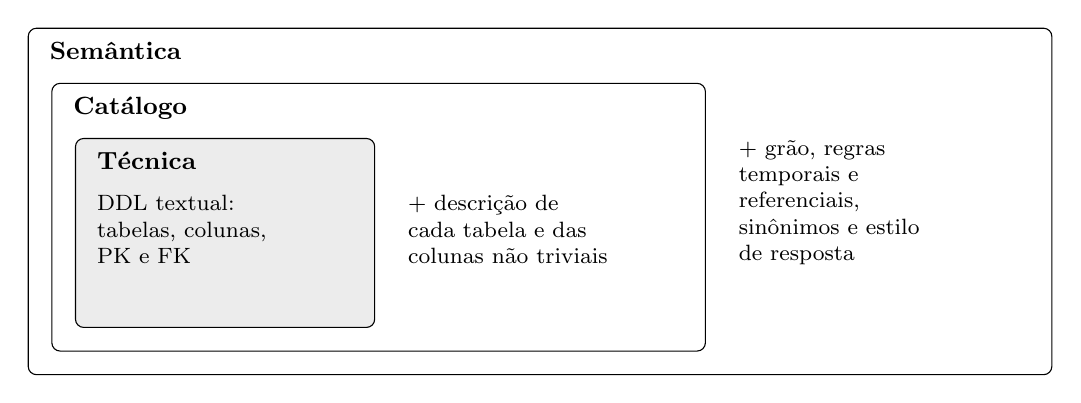
\begin{tikzpicture}[font=\small]
    % caixas aninhadas com coordenadas fixas (cm)
    \draw[rounded corners=3pt] (0,0) rectangle (13,4.4);
    \draw[rounded corners=3pt] (0.3,0.3) rectangle (8.6,3.7);
    \draw[rounded corners=3pt, fill=gray!15] (0.6,0.6) rectangle (4.4,3.0);
    \node[anchor=north west, font=\small\bfseries] at (0.15,4.35) {Semântica};
    \node[anchor=north west, font=\small\bfseries] at (0.45,3.65) {Catálogo};
    \node[anchor=north west, font=\small\bfseries] at (0.75,2.95) {Técnica};
    \node[anchor=north west, align=left, font=\footnotesize] at (0.75,2.4)
      {DDL textual:\\tabelas, colunas,\\PK e FK};
    \node[anchor=north west, align=left, font=\footnotesize] at (4.7,2.4)
      {+ descrição de\\cada tabela e das\\colunas não triviais};
    \node[anchor=north west, align=left, font=\footnotesize] at (8.9,3.1)
      {+ grão, regras\\temporais e\\referenciais,\\sinônimos e estilo\\de resposta};
  \end{tikzpicture}
  \fonte{Elaborado pelo autor.}
\end{figure}

As variáveis dependentes são:
\begin{alineas}
  \item \textbf{correção}, variável binária que indica se a consulta gerada
        executa e devolve o mesmo resultado da consulta de referência
        (\autoref{sec:avaliacao});
  \item \textbf{latência do modelo}, o tempo de parede da chamada ao
        provedor, em milissegundos (\autoref{sec:analise}).
\end{alineas}

Permanecem constantes entre as condições: o agente, o modelo, as perguntas,
o \textit{snapshot} da base de dados, os parâmetros de geração e o critério
de correção. A hipótese nula é a de que não há diferença de acurácia entre
as condições; a alternativa é bilateral, de forma que o estudo pode detectar
tanto melhora quanto piora.

% -----------------------------------------------------------------------------
\section{Fonte de dados}
\label{sec:fonte-dados}

\subsection{Seleção e autorização}
\label{sec:selecao-base}

Três conjuntos de dados candidatos foram avaliados localmente, apenas por
estrutura e estatísticas agregadas (contagens, cabeçalhos, tipos, nulos e
duplicidades), sem exposição de valores de linha. O resultado da avaliação
está resumido no \autoref{qua:bases}.

\begin{quadro}[htb]
  \centering
  \caption{Classificação das bases candidatas}
  \label{qua:bases}
  \begin{tabularx}{\textwidth}{|l|l|X|}
    \hline
    \textbf{Base} & \textbf{Classificação} & \textbf{Justificativa} \\ \hline
    Comercial & Usar com transformações & Autorização confirmada; 11 tabelas
      relacionadas; exige normalização de XLSX para PostgreSQL. \\ \hline
    Financeiro & Não usar & Autorização específica e privacidade não
      confirmadas. \\ \hline
    CSVs sintéticos fragmentados & Não usar & Não formam um
      \textit{snapshot} relacional íntegro. \\ \hline
  \end{tabularx}
  \fonte{Elaborado pelo autor a partir de \arq{artifacts/data_assessment/report.md}.}
\end{quadro}

A base escolhida, denominada \arq{commercial}, é um recorte comercial
descaracterizado. Em 26 de setembro de 2026, o responsável pelos dados
confirmou a descaracterização e autorizou o uso acadêmico local
(decisão D-001). A base financeira foi excluída por falta de confirmação
específica. Um conjunto sintético (\arq{synthetic_commercial}) foi mantido
apenas para os testes automatizados do código e não participa do
experimento.

A opção por uma base real descaracterizada, em vez de um \textit{benchmark}
acadêmico com esquema preparado para avaliação, é deliberada. A base carrega
características típicas de dados comerciais autênticos: referências órfãs
entre tabelas, datas registradas por extenso em português, nomes de coluna
que misturam termos de negócio e convenções técnicas, e medidas
monetárias em grãos diferentes. Essas características tornam o teto de
acurácia mais baixo, mas aproximam a medição do cenário em que agentes de
consulta são efetivamente empregados.

\subsection{Transformação para o modelo relacional}
\label{sec:transformacao}

As 11 planilhas XLSX de origem foram lidas sem modificação e normalizadas em
um esquema PostgreSQL com 11 tabelas, descritas no \autoref{qua:tabelas}.
As datas de emissão, registradas em português por extenso (por exemplo,
``terça-feira, 13 de dezembro de 2016''), foram convertidas para o tipo
\arq{date} durante a carga. Após a carga, a base contém 10.931 pedidos e
246.737 itens de pedido, com datas de emissão entre 18 de janeiro de 2016 e
26 de fevereiro de 2026.

\begin{quadro}[htb]
  \centering
  \caption{Tabelas do esquema \arq{commercial}}
  \label{qua:tabelas}
  \begin{tabularx}{\textwidth}{|l|l|X|}
    \hline
    \textbf{Tabela} & \textbf{Papel} & \textbf{Conteúdo e grão} \\ \hline
    \arq{orders} & Fato & Cabeçalho de pedido, uma linha por pedido \\ \hline
    \arq{order_items} & Fato & Item de pedido, N linhas por pedido \\ \hline
    \arq{targets} & Fato & Metas e realizado por representante e período \\ \hline
    \arq{customers} & Dimensão & Clientes \\ \hline
    \arq{representatives} & Dimensão & Representantes de vendas \\ \hline
    \arq{products} & Dimensão & Produtos cadastrados \\ \hline
    \arq{collections} & Dimensão & Coleções de produto, com vigência \\ \hline
    \arq{families} & Dimensão & Famílias de produto, agrupadas por coleção \\ \hline
    \arq{groups} & Dimensão & Grupos de classificação de produto \\ \hline
    \arq{subgroups} & Dimensão & Subgrupos, aninhados em grupos \\ \hline
    \arq{lines} & Dimensão & Linhas de produto \\ \hline
  \end{tabularx}
  \fonte{Elaborado pelo autor a partir de \arq{data/datasets/commercial/schema.sql}
    e \arq{catalog_context.sql}.}
\end{quadro}

\pendente{figura com diagrama entidade-relacionamento simplificado (opcional)}

O principal risco analítico do esquema é a relação de um para muitos entre
\arq{orders} e \arq{order_items}: somar uma medida do cabeçalho do pedido
após juntar os itens multiplica o valor pelo número de itens. Outro risco
é a coexistência de várias datas com semânticas distintas (emissão, entrega
prevista, cadastro de cliente, vigência de coleção e período de meta).

A primeira carga falhou porque a tabela \arq{subgroups} continha
referências a grupos inexistentes. Dados comerciais reais contêm
referências órfãs, e esse comportamento foi considerado parte do objeto de
estudo. Para preservar a fonte exatamente como autorizada, as declarações
\arq{REFERENCES} foram removidas do esquema (decisão D-004): as tabelas
mantêm nomes, tipos, chaves primárias e restrições \arq{NOT NULL}, mas o
PostgreSQL não valida a integridade referencial. A descrição textual das
relações (``FK $\rightarrow$ tabela'') continua sendo apresentada ao modelo.
A extensão do fenômeno é visível na tabela de pedidos: dos 10.931 pedidos
com cliente informado, 10.375 têm correspondência na tabela de clientes.

\subsection{Privacidade}
\label{sec:privacidade}

Nenhum valor de linha da base é enviado ao provedor do modelo
(decisão D-003). O modelo recebe apenas a descrição do esquema, o contexto
da condição e a pergunta. O agente não recebe amostras do resultado das
consultas que gera. Quando uma consulta
falha, o agente recebe somente a mensagem de erro de validação ou de
execução. A comparação entre o resultado gerado e o de referência é feita
localmente.

% -----------------------------------------------------------------------------
\section{Condições de contexto}
\label{sec:condicoes}

As três condições correspondem a três arquivos de texto mantidos sob
controle de versão e congelados por \textit{hash} (\autoref{sec:controles}).
O \autoref{qua:condicoes} resume o conteúdo de cada uma, e a
\autoref{tab:tamanho-contexto} mostra o tamanho do prompt resultante.

\begin{quadro}[htb]
  \centering
  \caption{Conteúdo de cada condição de contexto}
  \label{qua:condicoes}
  \begin{tabularx}{\textwidth}{|l|l|X|}
    \hline
    \textbf{Condição} & \textbf{Arquivo(s)} & \textbf{Conteúdo} \\ \hline
    Técnica & \arq{technical_context.sql} & Uma linha por tabela com colunas,
      chave primária e chaves estrangeiras (``FK $\rightarrow$ tabela''),
      sem descrições. \\ \hline
    Catálogo & \arq{catalog_context.sql} & O mesmo esquema, uma coluna por
      linha, com descrição de cada tabela e das colunas não triviais
      (valores monetários, contagens e datas), no formato de comentários
      de catálogo. \\ \hline
    Semântica & \arq{catalog_context.sql} + \arq{semantic_context.yaml} &
      O catálogo seguido do bloco ``SEMÂNTICA'', com: campos monetários e de
      contagem por tabela; regras de grão; regras temporais; regras
      referenciais; sinônimos em português; estilo de resposta. \\ \hline
  \end{tabularx}
  \fonte{Elaborado pelo autor a partir de \arq{data/datasets/commercial/}
    e \arq{src/tccsql/experiment/runner.py}.}
\end{quadro}

A condição técnica é análoga a fornecer ao modelo apenas a definição das
tabelas. A condição de catálogo é análoga aos comentários
\arq{COMMENT ON TABLE} e \arq{COMMENT ON COLUMN} mantidos em catálogos de
dados corporativos. A condição semântica é análoga a uma camada semântica,
que adiciona definições de métricas, grão, dimensões temporais e regras de
relacionamento. A correspondência entre cada seção do contexto semântico e
as ferramentas industriais é discutida na \autoref{sec:industriais}.

O contexto semântico é organizado em sete blocos:
\begin{alineas}
  \item \arq{money_fields} e \arq{count_fields}: definição de cada campo
        monetário e de contagem, por tabela;
  \item \arq{grain_rules}: o grão de cada tabela de fato e a proibição de
        somar \arq{orders.total_amount} após juntar os itens;
  \item \arq{temporal_rules}: qual coluna de data usar para emissão,
        entrega prevista, meta, vigência de coleção e cadastro de cliente;
  \item \arq{referential_rules}: o aviso de que há referências órfãs e a
        regra de usar \arq{IS NOT NULL} para ``Y informado'' e \arq{JOIN}
        para ``associado a Y existente'';
  \item \arq{synonyms}: termos de negócio em português (vendedor,
        representante, pedido, item, produto, faturamento) mapeados para
        tabelas e colunas;
  \item \arq{response_style}: devolver apenas as colunas pedidas,
        devolver um escalar quando não há agrupamento e não aplicar
        conversões de tipo desnecessárias;
  \item um cabeçalho com o domínio da base e a restrição de privacidade.
\end{alineas}
O conteúdo integral dos três contextos está no Apêndice~\ref{ap:contextos}.

\begin{table}[htb]
  \centering
  \caption{Tamanho do contexto por condição}
  \label{tab:tamanho-contexto}
  \begin{tabular}{lrrr}
    \toprule
    \multirow{2}{*}{Condição} & \multirow{2}{*}{Arquivo (bytes)} &
      \multicolumn{2}{c}{Tokens de entrada (mediana)} \\
    \cmidrule(lr){3-4}
     & & gpt-oss-120b & qwen3.8-27b \\
    \midrule
    Técnica   & 1.392 & 434 & 387 \\
    Catálogo  & 3.001 & 885 & 858 \\
    Semântica & 3.001 + 2.992 & 1.722 & 1.716 \\
    \bottomrule
  \end{tabular}
  \fonte{Elaborado pelo autor. Bytes dos arquivos em
    \arq{data/datasets/commercial/}; tokens de entrada informados pelo
    provedor em cada chamada, mediana sobre todas as tentativas das rodadas
    \arq{22e3f8ce} e \arq{07a25f55} (\arq{artifacts/raw/}).}
\end{table}

A descrição das colunas no catálogo e as definições dos campos no contexto
semântico se sobrepõem parcialmente. Essa sobreposição é intencional: o
nível semântico precisa conter todo o catálogo para que o desenho seja
aditivo, e a camada semântica de ferramentas industriais também repete
definições de campo ao lado das regras.

Um quarto arquivo do conjunto de dados, \arq{business_rules.yaml}, registra
as regras de negócio usadas na elaboração das perguntas e não é enviado ao
modelo em nenhuma condição.

% -----------------------------------------------------------------------------
\section{Agente de tradução para SQL}
\label{sec:agente}

O agente foi mantido deliberadamente simples para que o contexto fosse a
única fonte de variação. Ele faz uma única chamada ao modelo por tentativa,
sem exemplos (\textit{few-shot}), sem ferramentas, sem recuperação de
documentos e sem encadeamento de chamadas. O \textit{prompt} é composto por
uma mensagem de sistema fixa e uma mensagem de usuário com o contexto da
condição e a pergunta (\autoref{lst:prompt}).

\begin{lstlisting}[caption={Estrutura do \textit{prompt} enviado ao modelo},label={lst:prompt}]
[system]
Você é um agente text-to-SQL PostgreSQL. Responda somente com uma única
consulta SELECT ou WITH terminada em SELECT. Não explique.

[user]
ESQUEMA:
<contexto da condição: técnica, catálogo ou semântica>

PERGUNTA:
<pergunta em português>
SQL:
\end{lstlisting}
\fonte{\arq{src/tccsql/agent/text2sql.py}.}

O fluxo de execução de uma pergunta em uma condição é mostrado na
\autoref{fig:fluxo}. A resposta do modelo é reduzida ao bloco de código
SQL, quando presente, e passa por um validador sintático baseado na
biblioteca \textit{sqlglot}. O validador aceita uma única instrução, que
deve ser \arq{SELECT} ou \arq{WITH} terminado em \arq{SELECT}, rejeita
comandos de escrita e de definição de dados e restringe o acesso ao
esquema \arq{public}. A consulta validada é executada em uma transação
somente leitura, com um usuário de banco que possui apenas permissão de
leitura e tempo limite de 5 segundos por instrução.

\begin{figure}[htb]
  \centering
  \caption{Fluxo de execução de uma pergunta em uma condição}
  \label{fig:fluxo}
  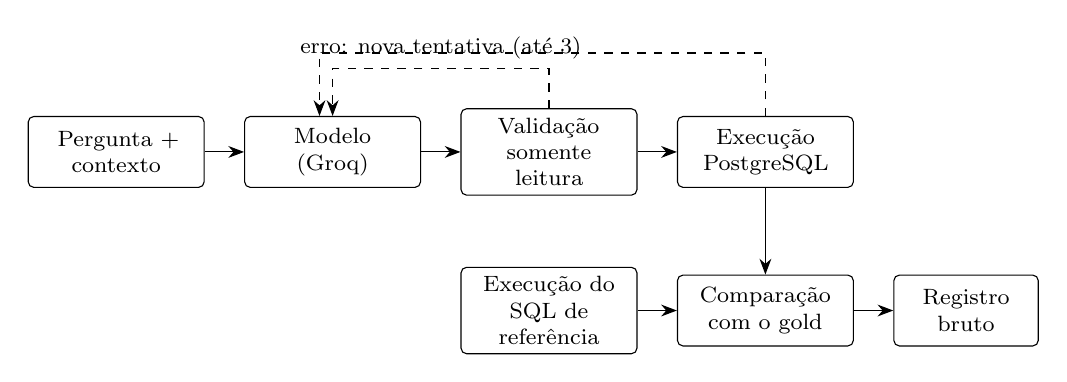
\begin{tikzpicture}[
      font=\footnotesize, node distance=0.45cm and 0.5cm,
      caixa/.style={draw, rounded corners=2pt, align=center, minimum height=0.9cm, text width=2.0cm},
      seta/.style={-{Stealth[length=2mm]}}]
    \node[caixa] (q) {Pergunta +\\contexto};
    \node[caixa, right=of q] (m) {Modelo\\(Groq)};
    \node[caixa, right=of m] (v) {Validação\\somente\\leitura};
    \node[caixa, right=of v] (e) {Execução\\PostgreSQL};
    \node[caixa, below=1.1cm of e] (c) {Comparação\\com o gold};
    \node[caixa, left=of c] (g) {Execução do\\SQL de\\referência};
    \node[caixa, right=0.5cm of c, text width=1.6cm] (r) {Registro\\bruto};
    \draw[seta] (q) -- (m);
    \draw[seta] (m) -- (v);
    \draw[seta] (v) -- (e);
    \draw[seta] (e) -- (c);
    \draw[seta] (g) -- (c);
    \draw[seta] (c) -- (r);
    \draw[seta, dashed] (v.north) -- ++(0,0.5) -| node[pos=0.25, above] {erro: nova tentativa (até 3)} (m.north);
    \draw[seta, dashed] (e.north) -- ++(0,0.8) -| (m.110);
  \end{tikzpicture}
  \fonte{Elaborado pelo autor a partir de \arq{src/tccsql/experiment/runner.py}.}
\end{figure}

Se a validação ou a execução falhar, o agente faz uma nova tentativa, até o
limite de três tentativas por pergunta e condição. A nova chamada repete a
mensagem de sistema e a mensagem com contexto e pergunta, acrescida de uma
mensagem com o erro técnico (``A tentativa anterior falhou tecnicamente:
\textit{erro}. Corrija e responda somente SQL.''). A consulta que falhou
não é reenviada ao modelo. Uma consulta que executa sem erro encerra as
tentativas, mesmo que o resultado esteja incorreto: o agente não recebe
nenhum sinal sobre a correção do resultado, apenas sobre falhas técnicas.

% -----------------------------------------------------------------------------
\section{Modelos e parâmetros}
\label{sec:modelos}

Foram usados dois modelos de pesos abertos de famílias distintas, ambos
servidos pela camada gratuita da API da Groq, compatível com a interface da
OpenAI (\autoref{tab:modelos}). O modelo principal é o
\arq{openai/gpt-oss-120b}. O \arq{qwen/qwen3.8-27b}, menor e de outra
família, foi adicionado para avaliar se o efeito depende do modelo
(decisão D-007). O identificador do modelo devolvido pelo provedor é gravado
em cada registro bruto.

\begin{table}[htb]
  \centering
  \caption{Modelos avaliados e parâmetros de geração}
  \label{tab:modelos}
  \begin{tabular}{lll}
    \toprule
    Item & Modelo principal & Réplica \\
    \midrule
    Identificador & \arq{openai/gpt-oss-120b} & \arq{qwen/qwen3.8-27b} \\
    Família & GPT-OSS (OpenAI) & Qwen (Alibaba) \\
    Parâmetros & 120 bilhões & 27 bilhões \\
    Provedor & Groq (camada gratuita) & Groq (camada gratuita) \\
    \arq{temperature} & 0 & 0 \\
    \arq{max_tokens} & 800 & 800 \\
    Rodada da coleta final & \arq{22e3f8ce} (16/11/2026) & \arq{07a25f55} (14/11/2026) \\
    \bottomrule
  \end{tabular}
  \fonte{Elaborado pelo autor a partir de \arq{src/tccsql/experiment/runner.py},
    \arq{docs/decisions.md} e \arq{artifacts/raw/}.}
\end{table}

\pendente{citar a fonte primária (model card) da contagem de parâmetros de cada modelo}

A temperatura zero reduz a variabilidade da geração, mas não a elimina:
o código não fixa semente (\textit{seed}) na requisição, e provedores de
inferência não garantem saída idêntica entre chamadas. Essa limitação é
discutida na \autoref{sec:validade}.

O uso de modelos abertos servidos gratuitamente é uma escolha de projeto:
o experimento inteiro roda sem custo financeiro e sem dependência de
plataformas proprietárias de dados ou de modelos, o que permite que
qualquer pesquisador o reproduza ou o estenda com outros modelos.

% -----------------------------------------------------------------------------
\section{Banco de perguntas}
\label{sec:perguntas}

O banco tem 50 perguntas em português: 40 para a coleta final e 10 para o
estudo piloto. Os enunciados dos dois conjuntos são distintos, embora três
perguntas do piloto tenham a mesma consulta de referência de perguntas
finais, com outra redação. As perguntas da coleta final se distribuem
igualmente em quatro categorias (\autoref{tab:perguntas}). Cada pergunta
tem identificador, categoria, enunciado, consulta SQL de referência
(\textit{gold}), tolerância numérica e um indicador de se a ordem das linhas
importa para a correção. Nas 40 perguntas finais, a tolerância é
$10^{-6}$ e a ordem das linhas não é considerada.

\begin{table}[htb]
  \centering
  \caption{Distribuição das perguntas por categoria}
  \label{tab:perguntas}
  \begin{tabularx}{\textwidth}{lccX}
    \toprule
    Categoria & Final & Piloto & Exemplo (coleta final) \\
    \midrule
    Filtros e agregações & 10 & 3 & ``Quantos clientes há na base?'' \\
    Relacionamentos & 10 & 3 & ``Quantos pedidos têm cliente associado?'' \\
    Temporal & 10 & 2 & ``Quantos pedidos foram emitidos em cada ano?'' \\
    Regras de negócio & 10 & 2 & ``Qual é o faturamento total no grão de pedido?'' \\
    \midrule
    Total & 40 & 10 & \\
    \bottomrule
  \end{tabularx}
  \fonte{Elaborado pelo autor a partir de \arq{questions_final.jsonl} e
    \arq{questions_pilot.jsonl}.}
\end{table}

\pendente{confirmar autoria e critério de elaboração das perguntas e das consultas de referência}

As perguntas e as consultas de referência são geradas por
\arq{scripts/question_bank.py} e congeladas por \textit{hash} antes de cada
coleta (\autoref{sec:controles}). A única alteração posterior à primeira
coleta final é a padronização descrita a seguir. A lista completa está no
Apêndice~\ref{ap:perguntas}.

Durante a auditoria da segunda execução final, identificou-se que
perguntas linguisticamente equivalentes sobre associação (``X têm Y
associado'', ``X estão associados a Y'') tinham consultas de referência
divididas entre \arq{JOIN} e \arq{WHERE y IS NOT NULL}, que produzem
resultados diferentes na presença de referências órfãs. As consultas de
referência de Q013, Q014 e Q016 foram padronizadas para \arq{JOIN},
alinhando-as a Q011, Q012, Q015 e Q017 (decisão D-006). O critério foi
estrutural: a forma da pergunta e a convenção já majoritária no banco, e não
a condição que seria favorecida.

% -----------------------------------------------------------------------------
\section{Controles experimentais}
\label{sec:controles}

Os seguintes controles foram aplicados em todas as execuções:
\begin{alineas}
  \item \textbf{pareamento}: em uma mesma rodada, cada pergunta é
        respondida nas três condições, uma após a outra;
  \item \textbf{contrabalanceamento}: a ordem das três condições segue uma
        das seis permutações possíveis, escolhida pelo índice da pergunta
        (índice módulo 6). Com 40 perguntas, quatro permutações são usadas
        sete vezes e duas são usadas seis vezes;
  \item \textbf{independência entre chamadas}: cada tentativa abre uma
        conversa nova, sem histórico de outras perguntas ou condições;
  \item \textbf{ausência de vazamento}: antes da execução, verifica-se que
        nenhuma consulta de referência aparece em nenhum contexto e que o
        bloco semântico não aparece nas condições técnica e de catálogo;
  \item \textbf{congelamento}: perguntas, esquema, contextos, regras e
        manifesto têm \textit{hash} SHA-256 registrado em
        \arq{checksums.sha256}; a execução é interrompida se algum arquivo
        tiver sido alterado;
  \item \textbf{rastreabilidade}: cada tentativa gera um registro
        imutável com pergunta, condição, ordem das condições, tentativa,
        modelo, SQL gerado, erro, tokens, latência, \textit{hash} do resultado
        e \textit{hash} dos três contextos.
\end{alineas}

A coleta final usa uma repetição por pergunta e condição (decisão D-002).
Com temperatura zero, repetições adicionais tenderiam a reproduzir as mesmas
respostas, e o poder estatístico vem das 40 perguntas pareadas.

% -----------------------------------------------------------------------------
\section{Critério de correção}
\label{sec:avaliacao}

Uma resposta é considerada correta quando a consulta gerada executa sem
erro e seu resultado é igual ao resultado da consulta de referência,
executada na mesma rodada e na mesma base. A comparação é feita sobre os
valores das linhas, sem considerar nomes de coluna, após uma normalização:
\begin{alineas}
  \item inteiros e decimais são tratados como números e arredondados à
        tolerância da pergunta;
  \item valores de data e hora à meia-noite são tratados como datas;
  \item quando a ordem não importa, as linhas são ordenadas antes da
        comparação.
\end{alineas}

As duas primeiras normalizações foram introduzidas após a primeira execução
final (decisão D-005), em que o avaliador tratava como diferentes valores
equivalentes, como o inteiro 2016 e o decimal 2016, e produzia falsos
negativos nas duas condições. A normalização não altera a exigência sobre
os valores.

O critério é conservador. Uma consulta semanticamente correta que devolve
colunas a mais, como o nome do representante ao lado do identificador,
é contada como erro. Por isso, a acurácia medida é um limite inferior da
acurácia que um avaliador humano atribuiria. Tentativas que esgotam as
três chamadas sem executar contam como erro.

% -----------------------------------------------------------------------------
\section{Análise estatística}
\label{sec:analise}

Para cada pergunta e condição, considera-se a última tentativa registrada.
A análise, implementada em \arq{scripts/analyze_results.py}, calcula:
\begin{alineas}
  \item a \textbf{acurácia} por condição, com intervalo de confiança de
        95\% pela aproximação normal da proporção;
  \item o \textbf{teste de McNemar exato} para cada um dos três pares de
        condições (técnica e catálogo, catálogo e semântica, técnica e
        semântica): o teste binomial bilateral sobre os pares discordantes,
        isto é, as perguntas acertadas em uma condição e erradas na outra;
  \item o \textbf{teste de postos sinalizados de Wilcoxon} pareado sobre a
        latência do modelo, para os mesmos três pares;
  \item o \textbf{ajuste de Holm} dos valores-p dentro de cada família de
        três comparações.
\end{alineas}

\pendente{citar referências para McNemar, Wilcoxon e o intervalo de confiança}

O teste de McNemar foi escolhido porque a correção é binária e as mesmas
perguntas são observadas em todas as condições: apenas os pares
discordantes informam sobre a diferença entre condições. Com 40 perguntas,
o intervalo de confiança pela aproximação normal é largo e deve ser lido
em conjunto com os testes pareados.

Adota-se nível de significância de 5\%. Como cada modelo envolve três
comparações pareadas, os valores-p de cada família de três testes são
ajustados pelo procedimento de Holm, que controla a taxa de erro por
família sem a perda de poder do ajuste de Bonferroni simples. Os
resultados apresentam o valor-p bruto e o ajustado lado a lado; a
significância é decidida pelo ajustado. O mesmo ajuste é aplicado aos
testes de latência.

\pendente{citar referência para o procedimento de Holm}

A latência do modelo é o tempo de parede entre o envio da requisição e o
recebimento da resposta, medido pelo cliente. Ela inclui as esperas de
retentativa que o cliente faz quando o provedor responde com limite de taxa
excedido (HTTP 429) ou erro temporário. Na camada gratuita, o limite de
tokens por minuto faz com que prompts maiores esperem mais. Assim, a
latência medida reflete o custo do prompt maior nas condições de uso deste
estudo, e não apenas o tempo de inferência do modelo.

% -----------------------------------------------------------------------------
\section{Trajetória metodológica}
\label{sec:trajetoria}

O protocolo definitivo resultou de uma sequência de decisões registradas,
cada uma com data, motivação e arquivo bruto preservado
(\autoref{qua:decisoes}). Os resultados de cada iteração são apresentados na
\autoref{sec:historico}.

\begin{quadro}[htb]
  \centering
  \caption{Decisões metodológicas}
  \label{qua:decisoes}
  \begin{tabularx}{\textwidth}{|l|X|X|}
    \hline
    \textbf{ID} & \textbf{Decisão} & \textbf{Motivação} \\ \hline
    D-001 & Usar a base comercial; excluir a financeira & Autorização
      específica para a primeira; privacidade na segunda \\ \hline
    D-002 & Pareamento, contrabalanceamento e uma repetição na coleta final
      & Temperatura zero torna repetições pouco informativas \\ \hline
    D-003 & Nenhum valor de linha enviado ao provedor & Privacidade \\ \hline
    D-004 & Esquema sem \arq{REFERENCES} & Preservar as referências órfãs
      da base real \\ \hline
    D-005 & Reescrever o contexto semântico e relaxar o avaliador quanto a
      tipos & Glossário genérico induzia erro; avaliador gerava falsos
      negativos \\ \hline
    D-006 & Padronizar o \textit{gold} das perguntas de associação em
      \arq{JOIN} & Inconsistência estrutural no banco de perguntas \\ \hline
    D-007 & Replicar no \arq{qwen/qwen3.8-27b} & Testar se o efeito depende
      do modelo \\ \hline
    D-008 & Adicionar a condição de catálogo & Separar o efeito das
      descrições de coluna do efeito das regras semânticas \\ \hline
  \end{tabularx}
  \fonte{Elaborado pelo autor a partir de \arq{docs/decisions.md}.}
\end{quadro}

O estudo começou com duas condições, técnica e semântica. Um estudo piloto
com 10 perguntas validou o fluxo de ponta a ponta. A primeira execução final
não mostrou diferença entre as condições, e a auditoria dos erros revelou
três problemas: um glossário semântico com sinônimo genérico, que induzia o
modelo a usar a coluna monetária errada; regras de relacionamento que
convidavam o modelo a acrescentar colunas descritivas não pedidas; e um
avaliador que penalizava diferenças de tipo sem diferença de valor. O
contexto semântico foi reescrito e o avaliador, ajustado (D-005). A
auditoria da segunda execução revelou a inconsistência nas consultas de
referência das perguntas de associação, corrigida em D-006.

Com o protocolo estabilizado, a coleta foi replicada em um segundo modelo
(D-007). Por fim, o desenho foi estendido para três condições (D-008), para
separar o efeito das descrições de coluna, que catálogos de dados já
oferecem, do efeito das regras próprias de uma camada semântica. Esse
desenho é o resultado principal deste trabalho.

As decisões D-005 e D-006 foram tomadas depois de observar erros da
coleta. Para limitar o viés do pesquisador, ambas seguiram critérios
estruturais: a reescrita do contexto foi feita por tabela e por tipo de
regra, e a padronização do \textit{gold} seguiu a forma linguística da
pergunta e a convenção já majoritária, e não o desempenho de uma condição
específica. Ainda assim, a possibilidade de viés é reconhecida na
\autoref{sec:validade}.

% -----------------------------------------------------------------------------
\section{Ambiente e reprodutibilidade}
\label{sec:reprodutibilidade}

O experimento é implementado em Python 3.12 e usa PostgreSQL 16 executado
em contêiner Docker. As principais bibliotecas são \textit{psycopg} para
acesso ao banco, \textit{sqlglot} para validação de SQL, \textit{pandas} e
\textit{SciPy} para a análise, e \textit{openpyxl} para a leitura das
planilhas. As etapas são encadeadas por um \textit{Makefile}: avaliação das
bases candidatas, preparação e carga do banco, testes automatizados, estudo
piloto, coleta final e análise.

Os registros brutos de cada execução são gravados em arquivos novos, nunca
sobrescritos, e os relatórios e tabelas derivados são gerados a partir
deles por \textit{script}. Dessa forma, todos os números apresentados na
\autoref{cap:resultados} podem ser recalculados a partir dos registros
brutos. Os arquivos XLSX de origem e os registros brutos não são
publicados, pois contêm ou derivam de dados da base.

\pendente{informar se o repositório será público e, se for, a URL a citar}

% =============================================================================
% 5 RESULTADOS — passo 3 da ordem.
% Números: SOMENTE de artifacts/reports/results_final_*-tiers.md e
% artifacts/processed/*-tiers.csv (3 níveis = resultado principal).
% gpt-oss-120b: run 22e3f8ce | qwen3.8-27b: run 07a25f55 (n = 40, regenerado).
% =============================================================================
\chapter{Resultados}
\label{cap:resultados}

\section{Estudo piloto}
\label{sec:piloto}
\begin{esboco}
  10 perguntas x 2 condições: 20/20 corretas, 1a tentativa (status.md).
  Função: validar o pipeline, não testar hipótese.
  PENDENTE: conferir em artifacts/raw/*_pilot_*.jsonl qual run citar.
\end{esboco}

\section{Acurácia por condição}
\label{sec:acuracia}
\begin{esboco}
  gpt-oss-120b: 62,5% -> 70,0% -> 82,5%, com IC 95%.
  qwen3.8-27b: 57,5% -> 60,0% -> 87,5%, com IC 95%.
  Tabela prevista: Tabela -- Acurácia por condição e modelo (n, acertos,
  acurácia, IC 95%).
  Figura prevista: Figura -- Acurácia por condição nos dois modelos
  (barras com IC).
\end{esboco}

\section{Comparações pareadas}
\label{sec:mcnemar}
\begin{esboco}
  McNemar exato, três pares por modelo (mcnemar_pairs_*-tiers.csv):
  gpt-oss: tech x cat 0:3 p=0,25; cat x sem 2:7 p=0,18; tech x sem 1:9 p=0,021.
  qwen:    tech x cat 1:2 p=1,0;  cat x sem 0:11 p=0,00098; tech x sem 0:12 p=0,00049.
  Tabela prevista: Tabela -- Pares discordantes e valor-p (McNemar exato).
\end{esboco}

\section{Acurácia por categoria de pergunta}
\label{sec:categorias}
\begin{esboco}
  by_category_*-tiers.csv (10 perguntas por categoria x condição).
  Tabela prevista: Tabela -- Acurácia por categoria, condição e modelo.
  Figura prevista: Figura -- Mapa de calor categoria x condição.
\end{esboco}

\section{Latência}
\label{sec:latencia}
\begin{esboco}
  Medianas e IQR (relatórios), Wilcoxon pareado.
  gpt-oss: ~1,4 s -> ~1,4 s -> ~7,9 s. qwen: ~2,9 s -> ~7,7 s -> ~14,8 s.
  Tabela prevista: Tabela -- Latência mediana do modelo por condição.
\end{esboco}

\section{Taxonomia de erros}
\label{sec:taxonomia}
\begin{esboco}
  docs/error_taxonomy.md: 16 perguntas com erro em algum nível (gpt-oss),
  7 classes (A a G), nível mínimo que resolve e seção do YAML responsável.
  NÃO usar os "6 pontos"/"9 pontos" do arquivo: não batem com as perguntas
  listadas. Recontar a partir de _failures_audit_tiers_gpt-oss.txt.
  PENDENTE: taxonomia equivalente para o qwen (não existe no repositório).
  Quadro previsto: Quadro -- Classes de erro, nível que resolve e seção do contexto.
  Figura prevista: Figura -- Decomposição do ganho por classe de erro.
\end{esboco}

\section{Exemplos qualitativos}
\label{sec:exemplos}
\begin{esboco}
  docs/qualitative_examples.md: Q005 (classe A), Q011 e Q013 (classe B/C),
  Q032 (A), Q038 (C). SQL de cada nível lado a lado.
  Cuidado: não reproduzir valores de linha além dos que já estão no doc.
  Quadros previstos: um por exemplo (pergunta, SQL por nível, correto/errado).
\end{esboco}

\section{Histórico: desenho com duas condições}
\label{sec:historico}
\begin{esboco}
  Desenho anterior (técnico x semântico), por iteração, gpt-oss:
  inicial 65,0% x 60,0% (p=1,0); pós-D-005 72,5% x 85,0% (p=0,18);
  pós-D-006 65,0% x 87,5% (p=0,0039). Réplica qwen: 55,0% x 85,0% (p=0,00049).
  Fontes: results_final_gpt-oss-120b.md, results_final_qwen3-27b.md,
  tabela "Histórico" de status.md com os arquivos brutos.
  Observação: o "semântico" de duas condições = técnico + YAML; no desenho
  de três = catálogo + YAML. Prompts diferentes, números não comparáveis 1:1.
  Tabela prevista: Tabela -- Evolução do resultado por iteração.
\end{esboco}

% =============================================================================
% 6 DISCUSSÃO — passo 4 da ordem.
% Fontes: docs/semantic_layer_mapping.md, docs/architecture.md (seção sobre
% garantia), docs/briefing.md §6-7, docs/error_taxonomy.md.
% =============================================================================
\chapter{Discussão}
\label{cap:discussao}

\section{Catálogo e camada semântica resolvem erros diferentes}
\label{sec:catalogo-vs-semantica}
\begin{esboco}
  Descrições de coluna resolvem escolha de coluna (classe A, G);
  só regras resolvem FK órfã (B) e colunas extras (C).
  Liga a taxonomia aos saltos medidos no Capítulo 5.
\end{esboco}

\section{Comparação com o benchmark da Databricks}
\label{sec:databricks}
\begin{esboco}
  40% -> 47% -> 97% (Databricks) vs 62,5 -> 70 -> 82,5 (gpt-oss) e
  57,5 -> 60 -> 87,5 (qwen). Mesmo formato: maior salto no último nível.
  Diferenças: base, perguntas, modelos, plataforma; não é réplica direta.
  PENDENTE: referência primária do benchmark.
  Tabela prevista: Tabela -- Comparação com o benchmark Databricks.
\end{esboco}

\section{Posicionamento frente às camadas semânticas industriais}
\label{sec:industriais}
\begin{esboco}
  Mapeamento seção do YAML -> dbt / Unity Catalog / LookML / Cube.
  response_style sem análogo (compilador resolve lá); referential_rules
  mais explícito aqui. Ponto: o metadado chega como texto no prompt em
  todas elas. "Piso" da camada semântica, sem ferramenta paga.
  Quadro previsto: Quadro -- Equivalência entre o contexto semântico e
  ferramentas industriais.
\end{esboco}

\section{Efeito maior no modelo menor}
\label{sec:modelo-menor}
\begin{esboco}
  qwen (27B): técnico 57,5% e semântico 87,5%; gpt-oss (120B): 62,5% e 82,5%.
  Salto técnico -> semântico maior no qwen (+30,0 pp vs +20,0 pp).
  Interpretação cautelosa (briefing §6.3): contexto compensa capacidade,
  com só dois modelos.
\end{esboco}

\section{O que garante o uso do contexto}
\label{sec:garantia}
\begin{esboco}
  architecture.md: nada estrutural; o YAML entra como texto e compete por
  atenção. Contexto semântico = engenharia de prompt sobre metadado, não
  camada de dados. Instruções ambíguas vazam (Q008 antes de D-005). Ganho
  estatístico, não garantia caso a caso.
\end{esboco}

\section{Custo em latência}
\label{sec:custo-latencia}
\begin{esboco}
  Semântico ~5,6x mais lento no gpt-oss e ~5,1x no qwen (medianas dos
  relatórios de três níveis). Custo real em produção.
\end{esboco}

\section{O projeto do experimento importa}
\label{sec:design-importa}
\begin{esboco}
  Contexto genérico e gold inconsistente escondem (ou invertem) o efeito:
  -5,0 pp na rodada inicial. Lição metodológica (briefing §6.1).
\end{esboco}

\section{Ameaças à validade}
\label{sec:ameacas}
\begin{esboco}
  briefing §7: n = 40; dois modelos; snapshot único; iteração sobre dados
  vistos (D-005, D-006); avaliador conservador; perguntas ambíguas
  (Q019, Q035, Q040). Organizar em validade interna, externa, de construto
  e de conclusão.
\end{esboco}

% =============================================================================
% 7 CONCLUSÃO — primeira versão (18/11/2026), escrita com a skill
% revisao-conclusoes-cientificas: só conclusões já demonstradas na
% Discussão, no presente, sem "tendências" (gpt-oss-120b: sem diferença
% significativa após Holm), sem especulação.
% Guia UECE p. 66: seção numerada.
% Fontes: monografia/textuais/06-discussao.tex; docs/briefing.md §7;
% docs/error_taxonomy.md (implicações).
% =============================================================================
\chapter{Conclusão}
\label{cap:conclusao}

Em agentes que geram SQL livremente a partir de uma descrição textual do
banco, o que aumenta a correção das consultas são as regras sobre como a
base deve ser consultada, e não as descrições do que cada coluna
significa. Descrições de catálogo resolvem a escolha entre colunas
parecidas, mas não alteram de forma significativa a acurácia do agente.
Regras de relacionamento e de formato da resposta resolvem os
erros mais frequentes, que produzem consultas válidas e respostas
erradas, e elevam a acurácia de forma significativa no
\arq{qwen3.8-27b}. No \arq{gpt-oss-120b}, as três condições não diferem
estatisticamente com o banco de 40 perguntas.

As regras que mais contam são as que tratam das imperfeições dos dados e
da forma da resposta: o tratamento de referências órfãs e a restrição às
colunas pedidas. Essas informações não pertencem a nenhuma coluna
específica e, por isso, não cabem em um catálogo de dados. Nas camadas
semânticas industriais, elas são garantidas pelo compilador que gera o
SQL; em um agente que escreve o SQL, precisam ser dadas como instrução.

A forma mais simples de camada semântica, um arquivo de texto anexado ao
prompt, basta para reproduzir o padrão relatado pela indústria com
plataformas proprietárias: o catálogo acrescenta pouco, e o maior ganho
vem da camada semântica. Avaliar e adotar esse tipo de contexto não exige
licença paga, catálogo proprietário nem modelo fechado: o estudo inteiro
roda com ferramentas abertas e modelos de pesos abertos servidos
gratuitamente, sobre uma base comercial real.

O contexto semântico atua como instrução, e não como garantia. Ele
aumenta a proporção de acertos, mas o modelo pode deixar de aplicar uma
regra presente, e um contexto mal especificado, como um sinônimo
genérico, pode piorar o resultado em vez de melhorá-lo. O efeito de uma camada
semântica depende, portanto, da precisão com que ela é escrita e da
consistência das consultas usadas para avaliá-la. Seu custo é um prompt
maior em cada chamada, que aumenta a latência e o consumo de tokens.

Os objetivos específicos foram atingidos: o protocolo pareado e
reprodutível foi construído sobre uma base real descaracterizada; as três
condições foram comparadas em dois modelos de famílias distintas, com
testes pareados e ajuste para comparações múltiplas; os erros foram
classificados e associados ao nível de contexto que os resolve; o custo
em latência foi medido; e o contexto semântico foi relacionado às
ferramentas industriais e ao benchmark da comunidade Databricks.

% -----------------------------------------------------------------------------
\section{Trabalhos futuros}
\label{sec:trabalhos-futuros}

Os resultados apontam quatro passos que decorrem diretamente das
limitações e dos achados deste estudo.

O primeiro é repetir o experimento com um banco de perguntas maior,
escrito por outras pessoas depois do congelamento do contexto. Um banco
maior aumenta o poder dos testes pareados, necessário para decidir se o
efeito existe no \arq{gpt-oss-120b}, e um banco escrito por terceiros
afasta a possibilidade de o vocabulário das regras ter sido ajustado ao
das perguntas. A mesma revisão deve tratar as perguntas cujo enunciado
admite mais de uma leitura (Q019, Q035 e Q040) e as convenções de tipo
temporal da classe D, que hoje limitam a acurácia máxima observável.

O segundo é comparar o contexto semântico textual com uma camada
semântica consultada por meio de um compilador, como as do dbt ou do
Cube. Os erros de referência órfã e de colunas extras, que mais
contribuem para o ganho, são evitados por construção nesse tipo de
arquitetura; a comparação mostraria quanto do ganho depende de o modelo
escrever o SQL.

O terceiro é estender o estudo a esquemas maiores, em que o contexto
inteiro não cabe no prompt. Nesse cenário, é preciso selecionar as
tabelas e as regras relevantes para cada pergunta, e a seleção passa a
ser parte do que se avalia, com efeito também sobre o custo em tokens e
a latência.

O quarto é incluir modelos de outros tamanhos e famílias, inclusive
modelos proprietários e modelos com menos de 10 bilhões de parâmetros,
para separar o efeito do tamanho do efeito da família, o que os dois
modelos avaliados aqui não permitem.


\postextual
\bibliography{referencias}

\begin{apendicesenv}
\partapendices
% Apêndices — material elaborado pelo autor (Guia UECE: pós-textuais opcionais).
% Numeração de páginas contínua.

\chapter{Banco de perguntas da coleta final}
\label{ap:perguntas}
\begin{esboco}
  40 perguntas com id, categoria e enunciado (questions_final.jsonl).
  PENDENTE: decidir se o gold SQL entra; conferir antes se algum gold tem
  literal com valor de linha da base (D-003).
\end{esboco}

\chapter{Contextos fornecidos ao modelo}
\label{ap:contextos}
\begin{esboco}
  Texto integral de technical_context.sql, catalog_context.sql e
  semantic_context.yaml (lstlisting). São metadados, sem valores de linha.
\end{esboco}

\chapter{Registro de decisões metodológicas}
\label{ap:decisoes}
\begin{esboco}
  D-001 a D-008 resumidas (docs/decisions.md), com data e arquivo bruto
  correspondente.
\end{esboco}

\end{apendicesenv}

\end{document}
